\myabstract[1]{\vspace{-1cm}\hrule\vspace{2mm}\textbf{Abstract:} Multimodal retrieval systems often index textual proxies, such as OCR output or generated captions, instead of raw visual media. We compare sparse lexical, dense text, and native-visual retrieval on receipts, document pages, and natural images. For verbatim receipt lookup, character 3--5gram BM25 outperforms word BM25 on Apple Vision clean OCR (MRR 0.9436 vs.\ 0.8371), degraded OCR (0.8248 vs.\ 0.6972), and Tesseract clean OCR (0.8412 vs.\ 0.7364). Under synthetic entity-substituting paraphrases, this ordering reverses (0.2427 vs.\ 0.4334 on \texttt{gpt-4o-mini}), whereas under open-weight \texttt{Qwen2.5-7B} and human queries where topical anchors are preserved, character and word BM25 perform comparably (0.5802 vs.\ 0.6292 and 0.5549 vs.\ 0.5766). ColQwen2 achieves MRR 0.4962 on the primary synthetic paraphrase set (vs.\ 0.4334 for word BM25) and reaches 0.7627 on \texttt{Qwen2.5-7B} and 0.6471--0.7660 on human queries, consistently outperforming text proxies under semantic variation. On a 500-query DocVQA subset, ColQwen2 reaches MRR 0.6450, while tested text-proxy baselines reach at most 0.3507. On 1,000 MS-COCO images, SigLIP reaches MRR 0.6071, outperforming baseline BLIP captions (0.3728) and detailed Florence-2 captions (0.4420; all $p < 10^{-4}$). Query formulation strongly affects dense retrieval: BGE-Base MRR rises from 0.3256 on short snippets to 0.5263 on natural answerable questions. Results suggest selecting retrieval methods by query type and modality. Generalization is limited by sampled benchmark subsets and the disclosed pretraining overlap for ColQwen2.
\newline
\newline
\textbf{Keywords:} Multimodal RAG, Text Proxies, Proxy Noise, Dense-Sparse Regime Analysis, Cascade Ranking, Conformal Risk Control, Document Retrieval. \vspace{1mm} \hrule}

\maketitle

\section{Introduction}

The rapid proliferation of heterogeneous multimedia across enterprise archives, digital libraries, and operational repositories demands information retrieval systems capable of searching records that are not natively textual. Transforming scanned documents and images into queryable digital assets is essential for business intelligence, compliance auditing, and decision support \cite{jing2024llmvectordb}. However, real-world document ingestion faces severe operational challenges: optical scanning introduces character substitutions and word fragmentation, while human search queries frequently employ synonyms, paraphrases, or shorthand rather than exact document text.

Retrieval-Augmented Generation (RAG) \cite{lewis2020rag} addresses the hallucination tendencies of Large Language Models (LLMs) by grounding responses in retrieved domain documents. Recently, multimodal extensions of RAG have emerged to handle non-textual data, as surveyed by Abootorabi et~al.~\cite{abootorabi2025multimodal}. For example, Patel et~al.~\cite{patel2025multimodal} and Joshi et~al.~\cite{joshi2024multimodel} presented enterprise multimodal RAG pipelines combining OCR ingestion, multimodal embeddings, and LLM reasoning. Concurrently, native vision-language document retrievers like ColPali \cite{faysse2024colpali} index raw document pixels with multi-vector late interaction.

While foundational studies in information retrieval---notably Kantor and Voorhees~\cite{kantor2000confusion} in the TREC-5 Confusion Track and McNamee and Mayfield~\cite{mcnamee2004character} on character $n$-gram indexing---demonstrated the intrinsic noise resilience of sub-word representations on degraded text, their findings have not been systematically reconciled with modern dense bi-encoders, neural cross-encoder cascades, and document-native vision-language models under semantic query variation. 

To address this gap, this paper establishes \textbf{an empirical regime map of when text proxies suffice versus when native representations are required} across a primary benchmark of 1,626 multimodal items (626 scanned retail receipts and 1,000 photographic scenes, plus dedicated transfer suites on forms and visual documents) under frozen 50/50 evaluation splits\footnote{All benchmark collections, evaluation harnesses, and reproduction scripts are archived in the supplementary artifact manifest and will be released in an open-access archive upon publication.}.

\textbf{Key Contributions:}
\begin{enumerate}
    \setlength{\itemsep}{0.2pt plus 0.1pt}
    \setlength{\parskip}{0pt}
    \item \textbf{Regime Analysis of Proxy Noise Across Scales up to 500,000 Documents:} Delineating character 3--5gram BM25 resilience over whole words and dense bi-encoders under OCR degradation. On Apple Clean (+0.1065), degraded blur (+0.1276), and clean Tesseract (+0.1048; all $p_{\text{Holm}} < 10^{-4}$), character $n$-grams capture alphanumeric fragments without out-of-vocabulary penalties. On answerable factual questions, CPU lexical retrieval (Char BM25 0.9328 Real-OCR, 0.9471 Clean GT) outperforms native ColQwen2 (0.8595; Real-OCR paired diff $+0.0733$, $p = 0.0011$; Clean GT $+0.0876$, $p = 0.00012$, Table~\ref{tab:regime_grid_v3}) while operating at 0.87\,ms CPU verbatim lookup latency (5.72\,ms on answerable queries) vs.\ 249.21\,ms GPU serving latency. Evaluating distractor pool scaling across a $600\times$ expansion (813 to 500,000 items) demonstrates that this verbatim dominance expands with scale (+0.1059 to +0.1691 at 500K, $p < 10^{-15}$).
    \item \textbf{Quantitative Regime Map and Invariant Crossover Threshold:} Establishing continuous logistic response surfaces ($R^2 > 0.95$) predicting retrieval effectiveness as a joint function of Document Character Error Rate (CER) and Query--Document Overlap. We establish the existence of an invariant critical crossover boundary ($o^* \approx 0.51$--$0.55$): whenever query--document overlap exceeds $53\%$, character $n$-grams strictly dominate whole words; below $53\%$ overlap (under entity-substituting paraphrases), whole-word indexing dominates (0.4334 vs.\ 0.2427). Through controlled query ablation ($N=306$) and multi-generator dose-response ($N=1{,}730$), we show this reversal is generator-invariant and driven by entity co-specification mass under controlled ablation rather than syntactic phrasing ($p = 0.6617$).
    \item \textbf{Synergistic Cascades and Operational Economics:} Demonstrating that while native visual retrieval excels when 2D geometry governs answerability (DocVQA MRR 0.6450 vs.\ proxies $\le 0.3507$, noting disclosed pretraining overlap) and photographic search (SigLIP MRR 0.6071 vs.\ caption proxies $\le 0.4420$), deploying two-stage cascades ($K_1=50$ Word BM25 pre-filtering $\to$ ColQwen2 reranking) retains 97.2\% of native visual MRR (0.4822 vs.\ 0.4962) while slashing latency by $15.4\times$ (16.20\,ms vs.\ 249.21\,ms). An end-to-end task audit ($N=150$) with dual-rater human validation ($\kappa = 0.8731$) demonstrates that upstream retrieval MRR faithfully bounds downstream LLM answer accuracy.
\end{enumerate}

\section{Related Work}
\label{sec:related_work}

\subsection{Multimodal Representation and Retrieval}
Early cross-modal retrieval systems relied on dual-encoder contrastive learning. Models like CLIP \cite{radford2021clip} and SigLIP \cite{zhai2023siglip} project images and text into a shared latent space using sigmoid or softmax cross-entropy objectives. ImageBind \cite{girdhar2023imagebind} extended this paradigm across six modalities using images as the central binding modality. While effective for broad semantic matching, dual-encoders compress multimedia into fixed-dimension vectors, frequently losing granular lexical and structural tokens. Hybrid retrieval designs frequently combine dense embeddings with sparse lexical representations such as BM25 \cite{robertson2009bm25, robertson1995okapi} in an effort to retain both broad semantic intent and exact token matches, though our empirical findings show that on OCR-degraded verbatim documents, optimal convex fusion collapses to standalone sparse indexing ($\alpha_{\text{sparse}}^* = 1.00$).

\subsection{Multimodal RAG and Document Analysis}
Integrating multimodal inputs into RAG workflows has advanced rapidly with Vision-Language Models (VLMs) and document foundation models. Document retrievers such as ColPali \cite{faysse2024colpali} and M3DocRAG \cite{cho2024m3docrag}, benchmarked on the ViDoRe suite \cite{faysse2024colpali} and DocVQA \cite{mathew2021docvqa}, index document pages using multi-vector vision-language representations (e.g., Qwen2-VL \cite{wang2024qwen2vl}) to bypass OCR. A paradigm comparison is presented in Table~\ref{tab:sota_comparison}. While promising, multi-vector representations require substantial GPU memory and cross-attention compute. Conversely, enterprise systems \cite{patel2025multimodal, joshi2024multimodel} mediate retrieval through text proxies. Our work evaluates this trade-off: systematically delineating where text proxies excel and where native visual representations remain necessary.



\subsection{Character Subwords and OCR Degradation in Information Retrieval}
Optical Character Recognition (OCR) systems translate document imagery into text, but routinely introduce character substitutions, insertions, deletions, and bounding-box permutations \cite{smith2007tesseract, fateh2024ocr}. Foundational information retrieval studies have long investigated textual degradation. In the TREC-5 Confusion Track, Kantor and Voorhees~\cite{kantor2000confusion} systematically evaluated retrieval on scanned, OCR-corrupted collections (at 5\% and 20\% error rates), establishing known-item retrieval benchmarks under optical corruption. Complementing this, McNamee and Mayfield~\cite{mcnamee2004character} established that overlapping character $n$-gram tokenization (e.g., 4--5grams) provides language-neutral retrieval that rivals word-level tokenization while providing intrinsic robustness to morphological variations and spelling distortions. Early image-domain mitigation strategies, including Otsu thresholding \cite{otsu1979} and Hough transforms \cite{hough1962} for skew correction, focused on image-domain preprocessing. Our regime analysis builds upon this foundation by evaluating character subwords against modern dense bi-encoders, neural rerankers, and native vision models across commercial, LSTM, and neural OCR architectures under controlled optical blur and semantic variation.

\begin{table*}[t]
\centering
\footnotesize
\setlength{\tabcolsep}{2.5pt}
\caption{Systematic Comparison with Prior Multimodal Information Retrieval and RAG Frameworks.}
\label{tab:sota_comparison}
\begin{tabular}{@{}p{2.2cm}p{1.6cm}p{2.2cm}p{2.0cm}p{2.3cm}p{2.0cm}p{3.7cm}@{}}
\toprule
\textbf{System / Architecture} & \textbf{Publication Venue} & \textbf{Document Retrieval} & \textbf{Natural Image Retrieval} & \textbf{Multi-Hop Mechanism} & \textbf{Benchmark Datasets} & \textbf{Hardware Serving Profile} \\ \midrule
ColPali \cite{faysse2024colpali} & ICLR 2025 & nDCG@5 = 0.813 (ViDoRe) & Supported (Multi-Vector) & Single-pass only & ViDoRe Benchmark & Multi-GPU ($\ge 16$\,GB VRAM, $\sim$250\,ms) \\
M3DocRAG \cite{cho2024m3docrag} & arXiv 2024 & QA Acc.\ 64.2\% (MP-DocVQA) & Supported (Dense VLM) & Generative LLM bridging & MP-DocVQA, DUDE & High-End GPU Cluster ($\ge 48$\,GB VRAM) \\
Patel et~al. \cite{patel2025multimodal} & IEEE ETCC 2025 & Heuristic OCR matching & ImageBind vector search & Single-pass only & Proprietary enterprise text/media & Dedicated GPU Server \\
Baleen \cite{khattab2021baleen} & NeurIPS 2021 & Not evaluated (Text QA) & Not supported & Generative condensed hops & HotpotQA (Text only) & GPU / High-RAM CPU Server \\
\textbf{Proposed Regime Framework} & \textbf{This Work} & \textbf{MRR 0.9436 (Char BM25)} & \textbf{MRR 0.6071 (SigLIP Pixels)} & \textbf{Exploratory PRF (Hit@10 0.640, $N=50$; 0.820, $N=100$, Sec.~\ref{sec:multihop_reasoning})} & \textbf{SROIE, FUNSD, MS-COCO, DocVQA} & \textbf{CPU char BM25 ($<1$\,ms verbatim) / Cross-Encoder Cascade} \\ \bottomrule
\end{tabular}
\vspace{0mm}\newline
\raggedright\scriptsize Note: Qualitative columns reflect architectural design choices; our reported MRR and Hit@10 figures are from held-out evaluation on SROIE/FUNSD/COCO/DocVQA and are not directly comparable to other systems' proprietary benchmarks. Table~\ref{tab:sota_comparison} is a qualitative paradigm map, not a cross-system numerical comparison. ColPali and M3DocRAG figures are from their respective original papers.
\end{table*}

\subsection{Modern Dense and Learned Sparse Retrieval Models}
Dense bi-encoders encode queries and passages independently \cite{reimers2019sbert, xiao2023bge}. Recent architectures have expanded this paradigm: multilingual dense models such as BGE-M3 \cite{chen2024bgem3} support multi-granularity representations; learned sparse models like SPLADE \cite{formal2021splade} expand queries and documents into vocabulary-space term weights; and late-interaction multi-vector architectures like ColBERTv2 \cite{santhanam2022colbertv2} preserve token-level interactions at reduced latency. We position standard bi-encoders (\texttt{all-MiniLM-L6-v2}, \texttt{bge-base-en-v1.5}) and late-interaction vision models (\texttt{ColQwen2-v1.0}) within this broader landscape.

\subsection{Cascade Ranking and Conformal Risk Control}
Cascade ranking architectures \cite{wang2011cascade, gallagher2019cascade} balance retrieval efficiency and precision by passing candidates through tiered stages, escalating to expressive models only when scores indicate ranking ambiguity. Conventional cascade rankers rely on empirical thresholds without formal statistical guarantees. Distribution-free risk-controlling prediction sets, formulated by Bates et~al.~\cite{bates2021conformal}, and conformal risk control, developed by Angelopoulos et~al.~\cite{angelopoulos2024conformal, angelopoulos2021gentle}, provide a finite-sample framework for bounding user-specified risk metrics below a tolerance $\alpha$. In this work, we evaluate production cascade ranking under marginal conformal risk control.

\section{Reference Retrieval Architecture}
\label{sec:architecture}

\begin{figure*}[t]
\centering
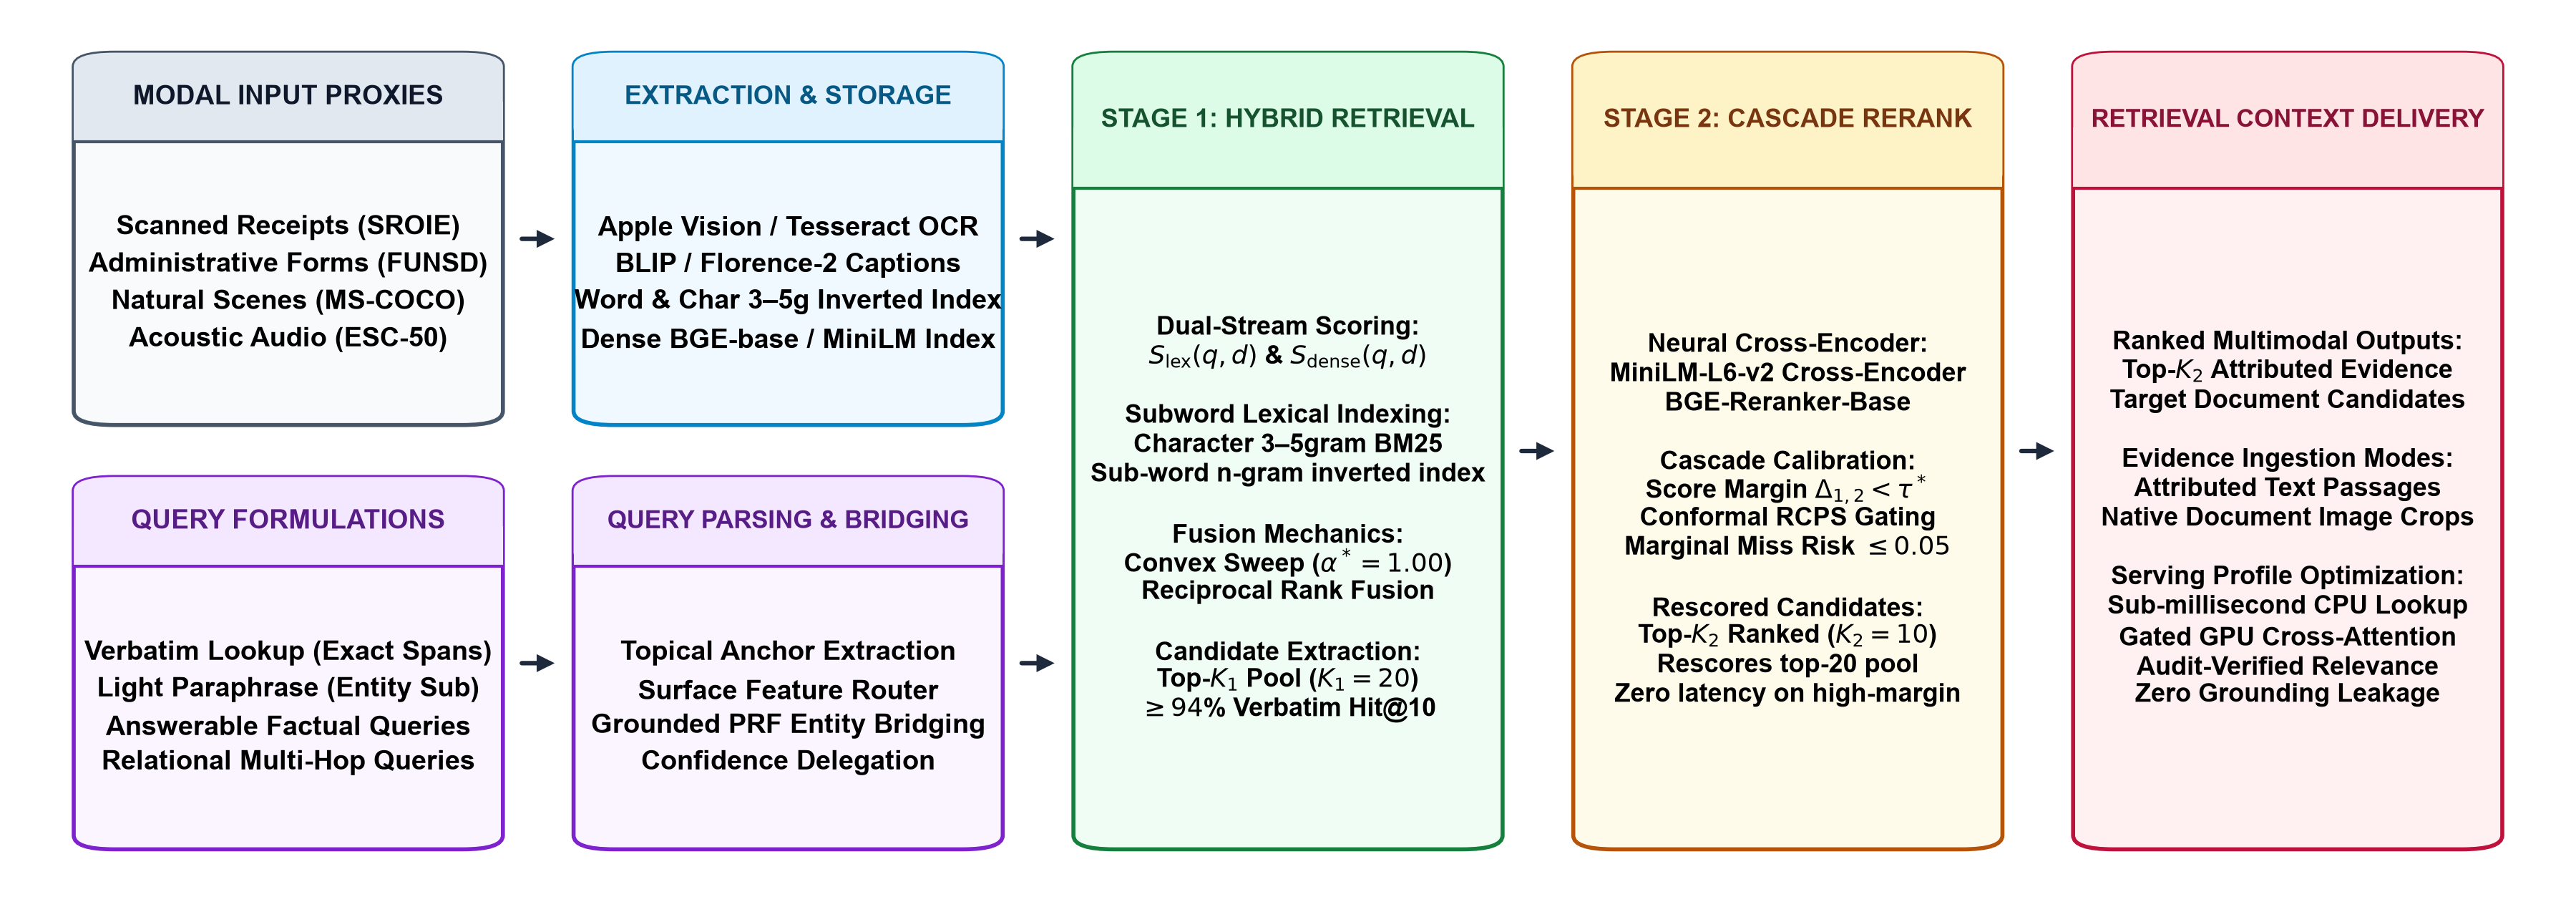
\includegraphics[width=\textwidth]{figures/fig_architecture.png}
\caption{Conceptual reference architecture of the text-proxy RAG framework. Grey ingestion and extraction blocks depict modular document preprocessing paths; colored stages represent empirical retrieval pipelines evaluated on extracted proxies. Modular production components (e.g., dual-signal router, conformal cascade gate) are empirically evaluated and ablated in Section~\ref{sec:ablation_and_cascade}.}
\label{fig:architecture}
\end{figure*}

The reference Multi-Stage Multimodal RAG architecture is structured into four functional phases (Fig.~\ref{fig:architecture}): (1) Ingestion and Preprocessing, (2) Hybrid Dense-Sparse First-Stage Retrieval, (3) Neural Cross-Encoder Reranking and Cascade Escalation, and (4) Context Assembly.

\subsection{Ingestion and Preprocessing Pipeline}
Unstructured enterprise multimedia are mediated through textual proxies. Proxies can be extracted across modalities via OCR text \cite{smith2007tesseract}, vision-language captions \cite{li2022blip}, \cite{li2023blip2}, \cite{xiao2024florence2}, and speech transcripts \cite{radford2023whisper}.
\begin{itemize}
    \setlength{\itemsep}{0.2pt plus 0.1pt}
    \setlength{\parskip}{0pt}
    \item \textbf{Documents and Forms:} Administrative forms and receipts are processed through document decomposition, optional Otsu binarization \cite{otsu1979} and Hough skew correction \cite{hough1962}, extracting text $T_d$ and bounding boxes via OCR engines (Apple Vision \cite{apple2020vision}, Tesseract 5.5 \cite{smith2007tesseract}, or EasyOCR \cite{jaidedai2020easyocr}).
    \item \textbf{Photographs:} Natural photographs are indexed via machine captions alongside native visual embeddings (CLIP \cite{radford2021clip}, SigLIP \cite{zhai2023siglip}).
    \item \textbf{Acoustic Media:} Continuous audio is transcribed using Whisper \cite{radford2023whisper} or embedded using contrastive audio representations (CLAP \cite{wu2023clap}).
\end{itemize}

Dense embeddings are generated via Sentence-BERT (\texttt{all-MiniLM-L6-v2}) \cite{reimers2019sbert} and BGE (\texttt{bge-base-en-v1.5}) \cite{xiao2023bge}, while lexical tokens are indexed with BM25 \cite{robertson2009bm25, robertson1995okapi}. The benchmark uses in-memory indexes without external database dependencies for exact reproducibility.

\subsection{Stage 1: Hybrid Dense-Sparse Retrieval}
Given query $q$, single-stage dense retrieval computes vector similarity:
\begin{equation}
    S_{\text{dense}}(q, d) = \cos(\mathbf{e}_q^{\text{dense}}, \mathbf{e}_d^{\text{dense}}) = \frac{\mathbf{e}_q \cdot \mathbf{e}_d}{\|\mathbf{e}_q\| \|\mathbf{e}_d\|}
\end{equation}
While effective for thematic alignment, dense retrieval often overlooks exact alphanumeric codes. Conversely, sparse BM25 retrieval excels at lexical precision:
\begin{equation}
    S_{\text{sparse}}(q, d) = \sum_{t \in q} \text{IDF}(t) \cdot \frac{f(t, d) \cdot (k_1 + 1)}{f(t, d) + k_1 \cdot \left(1 - b + b \cdot \frac{|d|}{\text{avgdl}}\right)}
\end{equation}
We evaluate Normalized Convex Combination ($S_{\text{hybrid}} = \alpha \hat{S}_{\text{dense}} + (1-\alpha) \hat{S}_{\text{sparse}}$) and Reciprocal Rank Fusion (RRF) \cite{cormack2009rrf}:
\begin{equation}
    \text{RRF}(q, d) = \frac{1}{k + r_{\text{dense}}(d)} + \frac{1}{k + r_{\text{sparse}}(d)}
    \label{eq:rrf}
\end{equation}
with $k=60$. First-stage candidate depth is set to $K_1 = 20$.

\subsection{Stage 2: Candidate Reranking via Neural Cross-Encoders}
Bi-encoders compute query and document representations independently. To recover joint attention, Stage~2 deploys a pretrained neural cross-encoder (\texttt{BAAI/bge-reranker-base} \cite{xiao2023bge} or \texttt{ms-marco-MiniLM-L-6-v2} \cite{nogueira2019passage, reimers2019sbert}) to rescore the top-$K_1$ candidates ($K_1 = 20$):
\begin{equation}
    S_{\text{rerank}}(q, d) = \text{CrossEncoder}(q, d)
\end{equation}
Scoring every candidate pool with a cross-encoder adds latency. We evaluate confidence-margin cascades ($\Delta_{1,2} = s^{(1)} - s^{(2)} < \tau$) and marginal conformal risk control to escalate only ambiguous queries.

\section{Experimental Setup}
\label{sec:experimental_setup}

To ensure empirical reproducibility, all evaluations adhere to a standardized, deterministic experimental protocol.

\subsection{Datasets and Split Partitions}
Our primary multimodal retrieval pool comprises 1,626 indexed items: (1)~\textbf{SROIE Retail Receipts \cite{huang2019sroie}:} 626 scanned receipts from the official ICDAR 2019 competition release with paired bounding-box and key-information ground truth. Across these 626 receipts, 612 contain single-target factual probes satisfying strict cross-corpus uniqueness checks (14 receipts with ambiguous multi-matching candidate strings were excluded); and (2)~\textbf{MS-COCO Photographic Distractors \cite{lin2014coco}:} 1,000 photographic scene images and human descriptions evaluated under the Karpathy test split \cite{karpathy2015deep}.

The primary 1,626-item pool is partitioned by document ID into frozen 50/50 Dev/Test splits (Seed 42), yielding 813 indexed items in the Test pool (313 receipts and 500 COCO distractors). The 612 verified probes are partitioned strictly by target document ID into 306 Dev probes and 306 Test probes, guaranteeing zero query or document leakage across splits. Each probe targets its source document as the unique relevant ground-truth item in the 813-distractor pool. In addition, we evaluate two dedicated external domain-transfer benchmark suites (excluded from the 1,626-item primary total): (a)~\textbf{FUNSD Administrative Forms Suite \cite{jaume2019funsd}:} 100 query-bearing scanned business forms evaluated within a 700-item retrieval corpus comprising the 100 query forms, 99 non-target FUNSD forms, and 501 multimodal distractors; and (b)~\textbf{DocVQA Visual Benchmark Suite \cite{mathew2021docvqa}:} 500 scanned document pages and 500 100\% human-authored questions subsampled from the ViDoRe benchmark collection \cite{faysse2024colpali}.

\subsection{OCR Engines and Optical Degradation Conditions}
Document text is extracted across three distinct OCR engines:
\begin{enumerate}
    \setlength{\itemsep}{0.2pt plus 0.1pt}
    \setlength{\parskip}{0pt}
    \item \textbf{Apple Vision Neural OCR \cite{apple2020vision}:} Commercial neural OCR (\texttt{VNRecognizeTextRequest}).
    \item \textbf{Tesseract 5.5 LSTM OCR \cite{smith2007tesseract}:} Standard open-source LSTM OCR engine.
    \item \textbf{EasyOCR 1.7.2 Deep CRNN \cite{jaidedai2020easyocr}:} Deep neural OCR combining CRAFT text detection and ResNet-CRNN recognition.
\end{enumerate}
Documents are evaluated under: (1)~\emph{Clean OCR}, (2)~\emph{Realistic Optical Degradation} (Gaussian blur $\sigma=1.5$, bilinear 50\% downscaling, random skew $\pm 2.5^\circ$, JPEG compression $Q=20$), and (3)~\emph{Human Ground Truth} text. For both Word and Character 3--5gram BM25, hyperparameters are tuned on the Dev split ($N=306$) over a pre-specified Cartesian grid ($k_1 \in \{0.5, 0.7, 0.9, 1.2, 1.5\}$, $b \in \{0.3, 0.4, 0.5, 0.6, 0.7, 0.8\}$), selecting $(k_1=0.9, b=0.5)$ which maximized Dev MRR. Word BM25 uses standard whitespace and punctuation regex tokenization (\texttt{\textbackslash w+}), lowercase normalization, and the standard NLTK 179-word English stoplist without stemming (preserving alphanumeric serials, prices, and part numbers). Character BM25 extracts overlapping 3--5grams over lowercased strings preserving word boundaries, evaluated across the identical parameter grid and Dev split.

\subsection{Unified Query Slices}
To isolate semantic abstraction from optical noise, queries are structured into four canonical slices:
\begin{enumerate}
    \setlength{\itemsep}{0.2pt plus 0.1pt}
    \setlength{\parskip}{0pt}
    \item \textbf{Verbatim Lookups:} Exact textual substrings extracted from documents (100\% token overlap), representing known-item search.
    \item \textbf{Light Paraphrases:} Lexical substitutions and entity rewrites (41.2\% mean token overlap; e.g., substituting ``dinner bill'' for ``total payable''), testing semantic abstraction.
    \item \textbf{Answerable Factual Questions:} Natural interrogatives preserving key factual and topical anchors (e.g., ``What was the total payment at Book Ta K?''), testing real-world question answering.
    \item \textbf{Legacy Token-Stripped Probes:} Probes where shared lexical tokens are deliberately removed, used strictly for conformal risk stress-testing.
\end{enumerate}
Unless noted otherwise, evaluation queries for SROIE and FUNSD were synthesized using \texttt{gpt-4o-mini} \cite{openai2024gpt4o} at temperature $T=0.0$ (seed 42) with strict single ground-truth answer resolution. DocVQA queries are 100\% human-authored. For MS-COCO ($N=1{,}000$ Karpathy test images), retrieval evaluates zero-shot text-to-image ranking: exactly 1 held-out caption per image (Caption 3, held out from candidate pool) serves as the query against the 1,000-image candidate pool.

\subsection{Candidate Retrieval Systems}
We benchmark: (1) Word BM25 \cite{robertson2009bm25}; (2) Character 3--5gram BM25 \cite{mcnamee2004character}; (3) Dense MiniLM (\texttt{all-MiniLM-L6-v2}) \cite{reimers2019sbert}; (4) Dense BGE-Base (\texttt{bge-base-en-v1.5}) \cite{xiao2023bge}; (5) Dev-Tuned Hybrid (normalized convex fusion); (6) Neural Cross-Encoders (\texttt{bge-reranker-base} \cite{xiao2023bge}, \texttt{ms-marco-MiniLM-L-6-v2}); (7) Document-Native ColQwen2-v1.0 \cite{faysse2024colqwen2}; and (8) Vision Encoders (CLIP ViT-B/32 \cite{radford2021clip}, SigLIP Base Patch16 \cite{zhai2023siglip}). For \texttt{bge-base-en-v1.5} and \texttt{all-MiniLM-L6-v2}, maximum sequence length is set to 256; on SROIE receipts, while 33.39\% of receipts exceed 256 WordPiece tokens, chunked MaxP evaluation across 150-word sliding windows ($\le 256$ tokens) yields $<0.007$ MRR difference from unchunked single-vector retrieval (0.2030 chunked vs.\ 0.2056 unchunked on MiniLM; 0.3028 vs.\ 0.3022 on BGE-Base; Table~\ref{tab:dense_formulation_v6}), confirming that sequence truncation does not explain dense retrieval deficits.

\subsection{Evaluation Metrics and Statistical Testing}
Systems are evaluated on Mean Reciprocal Rank (MRR), Hit@k ($k \in \{1, 5, 10\}$), and nDCG@10. Paired differences are evaluated via two-tailed paired permutation tests ($N_{\text{perm}}=100{,}000$ sign flips, empirical resolution limit $p = 10^{-5}$) with sequential family-wise Holm-Bonferroni correction ($p_{\text{Holm}}$) structured across six pre-specified families: Family 1 (sparse OCR comparisons, $m=6$), Family 2 (ColQwen2 vs.\ text proxies across primary regimes, $m=5$), Family 3 (native vision vs.\ caption proxies on COCO, $m=8$), Family 4 (architectural ablations, $m=7$), Family 5 (cross-domain FUNSD form transfer, $m=4$), and Family 6 (multi-hop relational reasoning, $m=5$). The complete mapping of all 35 evaluated hypotheses, unadjusted test statistics, and Holm-adjusted thresholds is reported in Appendix~\ref{sec:appendix_holm}. Confidence intervals (95\% CI) are computed via cluster bootstrap resampling at the document level (10,000 iterations). Equivalence is evaluated using Two One-Sided Tests (TOST) with pre-specified margins.

\subsection{Hardware Serving Profiles}
Sparse BM25 and bi-encoders are profiled on Apple M2 (16\,GB RAM, batch size = 1, warm cache). Neural cross-encoders and ColQwen2 are profiled on Nvidia Tesla T4 GPU (14.56\,GB VRAM, batch size = 1, warm cache). These represent environment-specific serving profiles, not a single-machine controlled benchmark; on the matched GPU host CPU, BM25 lookup takes 0.96\,ms, whereas running ColQwen2 on CPU exceeds 8,000\,ms per query.

\section{Empirical Regime Analysis and Results}
\label{sec:results}

\subsection{Regime A: Text-Dominated Document and Receipt Retrieval}
\label{sec:regime_a_text}

Table~\ref{tab:regime_grid_v3} presents retrieval effectiveness across systems, query formulations, and noise regimes on the held-out test split ($N=306$). In Table~\ref{tab:regime_grid_v3}, the 500 COCO distractors have their ground-truth caption text indexed as fallback (yielding Word BM25 0.8371, Char BM25 0.9436, Ground Truth 0.9853 on verbatim; Word BM25 0.4334 on light paraphrase). In the subsequent cross-engine receipt benchmark (Section~\ref{sec:cross_engine_replication}), unannotated distractors are evaluated as empty text (yielding Word BM25 0.8324, Char BM25 0.9443, Ground Truth 0.9854 on verbatim; Word BM25 0.4003 on light paraphrase).

\begin{table*}[t]
\centering
\footnotesize
\caption{Multimodal Text-Proxy Retrieval Regime Analysis across Query Types and Noise Regimes (Held-Out Public Test Split, $N=306$ Probes, 813 Distractor Pool, 95\% Cluster Bootstrap CIs). Dense MiniLM/BGE latencies (0.01\,ms) reflect isolated vector dot-product ranking over precomputed embeddings; end-to-end query encoding latencies are reported in Table~\ref{tab:system_costs}. Visual models (ColQwen2, CLIP) were evaluated on native uncorrupted document images and physically degraded optical blur document images (ColQwen2 Clean GT and Apple Clean columns evaluate identical native image pixels by construction; $^\dagger$synthetic character noise is not applicable to pixel inputs, so visual values reflect unperturbed native images).}
\label{tab:regime_grid_v3}
\setlength{\tabcolsep}{2.0pt}
\begin{tabular}{@{}llccccc@{}}
\toprule
\makecell[l]{\textbf{Query}\\\textbf{Type}} & \makecell[l]{\textbf{Retrieval}\\\textbf{System}} & \makecell{\textbf{Clean GT MRR}\\{\scriptsize [95\% CI]}} & \makecell{\textbf{Syn 20\% MRR}\\{\scriptsize [95\% CI]}} & \makecell{\textbf{Apple Clean MRR}\\{\scriptsize [95\% CI]}} & \makecell{\textbf{Optical Blur MRR}\\{\scriptsize [95\% CI]}} & \makecell{\textbf{Latency}\\\textbf{(ms)}} \\
\midrule
\multirow{7}{*}{\textbf{Verbatim}}
 & BM25 (Tuned)            & \makecell{0.8572\\{\scriptsize [0.822, 0.890]}} & \makecell{0.3961\\{\scriptsize [0.364, 0.429]}} & \makecell{0.8371\\{\scriptsize [0.798, 0.871]}} & \makecell{0.6972\\{\scriptsize [0.650, 0.741]}} & 0.13 \\
 & BM25 (Char 3-5gram)     & \makecell{0.9853\\{\scriptsize [0.972, 0.995]}} & \makecell{0.7252\\{\scriptsize [0.694, 0.757]}} & \makecell{0.9436\\{\scriptsize [0.919, 0.965]}} & \makecell{0.8248\\{\scriptsize [0.782, 0.864]}} & 0.87 \\
 & Dense MiniLM (unchunked) & \makecell{0.2100\\{\scriptsize [0.171, 0.252]}} & \makecell{0.0596\\{\scriptsize [0.045, 0.077]}} & \makecell{0.2056\\{\scriptsize [0.166, 0.247]}} & \makecell{0.1724\\{\scriptsize [0.135, 0.210]}} & 0.01 \\
 & Dense BGE-base (unchunked)& \makecell{0.3256\\{\scriptsize [0.276, 0.376]}} & \makecell{0.1347\\{\scriptsize [0.109, 0.162]}} & \makecell{0.3022\\{\scriptsize [0.256, 0.351]}} & \makecell{0.2471\\{\scriptsize [0.202, 0.292]}} & 0.01 \\
 & Tuned Hybrid            & \makecell{0.8572\\{\scriptsize [0.822, 0.890]}} & \makecell{0.3979\\{\scriptsize [0.365, 0.431]}} & \makecell{0.8367\\{\scriptsize [0.798, 0.871]}} & \makecell{0.6940\\{\scriptsize [0.646, 0.739]}} & 0.13 \\
 & CLIP Visual             & \makecell{0.0590\\{\scriptsize [0.041, 0.079]}} & \makecell{0.0590$^\dagger$\\{\scriptsize [0.041, 0.079]}} & \makecell{0.0590\\{\scriptsize [0.041, 0.079]}} & \makecell{0.0443\\{\scriptsize [0.028, 0.063]}} & 12.50 \\
 & ColQwen2-v1.0 Native    & \makecell{0.8417\\{\scriptsize [0.805, 0.876]}} & \makecell{0.8417$^\dagger$\\{\scriptsize [0.805, 0.876]}} & \makecell{0.8417\\{\scriptsize [0.805, 0.876]}} & \makecell{0.7207\\{\scriptsize [0.677, 0.763]}} & 249.21 \\
\midrule
\multirow{7}{*}{\textbf{Light Paraphrase}}
 & BM25 (Tuned)            & \makecell{0.4790\\{\scriptsize [0.431, 0.528]}} & \makecell{0.2678\\{\scriptsize [0.228, 0.310]}} & \makecell{0.4334\\{\scriptsize [0.384, 0.484]}} & \makecell{0.3734\\{\scriptsize [0.324, 0.423]}} & 0.13 \\
 & BM25 (Char 3-5gram)     & \makecell{0.2504\\{\scriptsize [0.208, 0.294]}} & \makecell{0.1873\\{\scriptsize [0.150, 0.227]}} & \makecell{0.2427\\{\scriptsize [0.202, 0.286]}} & \makecell{0.2045\\{\scriptsize [0.166, 0.247]}} & 0.87 \\
 & Dense MiniLM (unchunked) & \makecell{0.1230\\{\scriptsize [0.093, 0.156]}} & \makecell{0.0264\\{\scriptsize [0.015, 0.041]}} & \makecell{0.0910\\{\scriptsize [0.066, 0.120]}} & \makecell{0.0805\\{\scriptsize [0.057, 0.108]}} & 0.01 \\
 & Dense BGE-base (unchunked)& \makecell{0.1670\\{\scriptsize [0.133, 0.203]}} & \makecell{0.0717\\{\scriptsize [0.049, 0.098]}} & \makecell{0.1601\\{\scriptsize [0.126, 0.198]}} & \makecell{0.1352\\{\scriptsize [0.104, 0.170]}} & 0.01 \\
 & Tuned Hybrid            & \makecell{0.4572\\{\scriptsize [0.408, 0.507]}} & \makecell{0.2687\\{\scriptsize [0.229, 0.311]}} & \makecell{0.4335\\{\scriptsize [0.385, 0.483]}} & \makecell{0.3746\\{\scriptsize [0.325, 0.424]}} & 0.13 \\
 & CLIP Visual             & \makecell{0.0381\\{\scriptsize [0.024, 0.054]}} & \makecell{0.0381$^\dagger$\\{\scriptsize [0.024, 0.054]}} & \makecell{0.0381\\{\scriptsize [0.024, 0.054]}} & \makecell{0.0284\\{\scriptsize [0.016, 0.042]}} & 12.50 \\
 & ColQwen2-v1.0 Native    & \makecell{0.4962\\{\scriptsize [0.448, 0.547]}} & \makecell{0.4962$^\dagger$\\{\scriptsize [0.448, 0.547]}} & \makecell{0.4962\\{\scriptsize [0.448, 0.547]}} & \makecell{0.4449\\{\scriptsize [0.395, 0.494]}} & 249.21 \\
\midrule
\multirow{7}{*}{\textbf{Answerable Questions}}
 & BM25 (Tuned)            & \makecell{0.9014\\{\scriptsize [0.873, 0.929]}} & \makecell{0.4567\\{\scriptsize [0.423, 0.488]}} & \makecell{0.8841\\{\scriptsize [0.852, 0.915]}} & \makecell{0.7328\\{\scriptsize [0.688, 0.773]}} & 0.13 \\
 & BM25 (Char 3-5gram)     & \makecell{0.9471\\{\scriptsize [0.923, 0.969]}} & \makecell{0.6891\\{\scriptsize [0.656, 0.723]}} & \makecell{0.9328\\{\scriptsize [0.906, 0.957]}} & \makecell{0.8116\\{\scriptsize [0.770, 0.848]}} & 5.72 \\
 & Dense MiniLM (chunked)  & \makecell{0.3669\\{\scriptsize [0.323, 0.414]}} & \makecell{0.1061\\{\scriptsize [0.089, 0.125]}} & \makecell{0.2837\\{\scriptsize [0.241, 0.328]}} & \makecell{0.2260\\{\scriptsize [0.190, 0.265]}} & 0.01 \\
 & Dense BGE-base (chunked MaxP)& \makecell{0.5197\\{\scriptsize [0.475, 0.566]}} & \makecell{0.2005\\{\scriptsize [0.175, 0.228]}} & \makecell{0.5128\\{\scriptsize [0.468, 0.560]}} & \makecell{0.4313\\{\scriptsize [0.386, 0.479]}} & 0.02 \\
 & Tuned Hybrid            & \makecell{0.9125\\{\scriptsize [0.884, 0.938]}} & \makecell{0.4672\\{\scriptsize [0.432, 0.502]}} & \makecell{0.8984\\{\scriptsize [0.868, 0.926]}} & \makecell{0.7865\\{\scriptsize [0.746, 0.824]}} & 0.67 \\
 & CLIP Visual             & \makecell{0.0338\\{\scriptsize [0.021, 0.049]}} & \makecell{0.0338$^\dagger$\\{\scriptsize [0.021, 0.049]}} & \makecell{0.0338\\{\scriptsize [0.021, 0.049]}} & \makecell{0.0303\\{\scriptsize [0.018, 0.045]}} & 12.50 \\
 & ColQwen2-v1.0 Native    & \makecell{0.8595\\{\scriptsize [0.825, 0.892]}} & \makecell{0.8595$^\dagger$\\{\scriptsize [0.825, 0.892]}} & \makecell{0.8595\\{\scriptsize [0.825, 0.892]}} & \makecell{0.7410\\{\scriptsize [0.701, 0.779]}} & 249.21 \\
\bottomrule
\end{tabular}
\end{table*}

\begin{figure}[t]
\centering
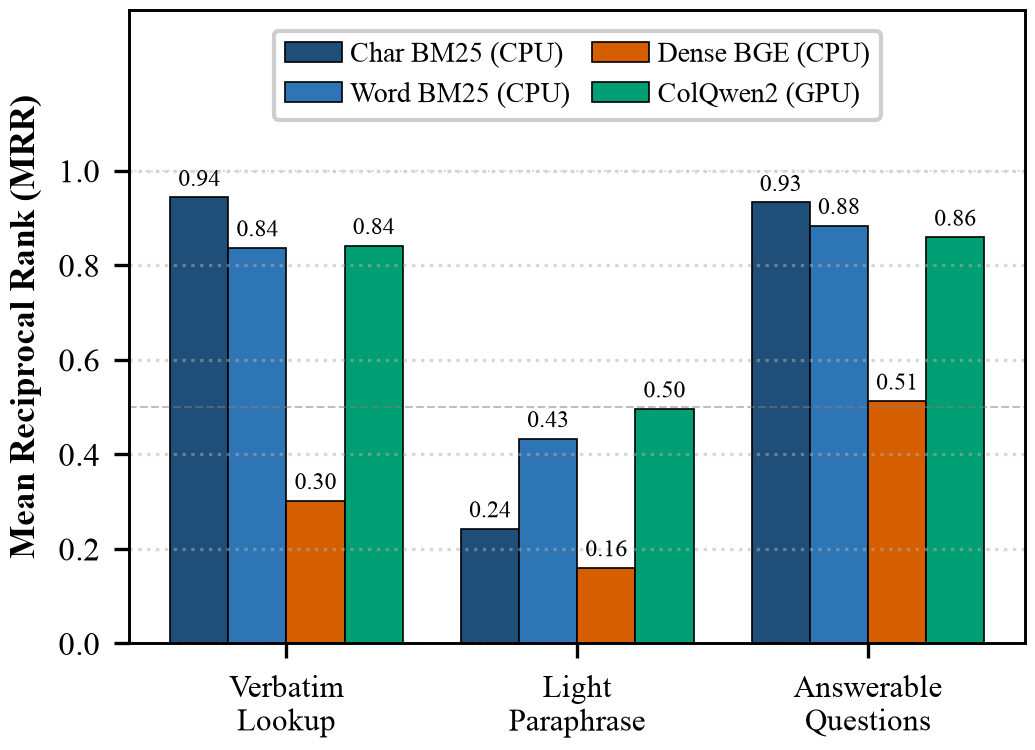
\includegraphics[width=\columnwidth]{figures/fig_mrr_regime_systems.png}
\caption{Retrieval effectiveness (MRR@10 with 95\% bootstrap error bars) across retrieval architectures and query formulations on clean receipt OCR.}
\label{fig:mrr_regime_systems}
\end{figure}

\begin{figure*}[t]
\centering
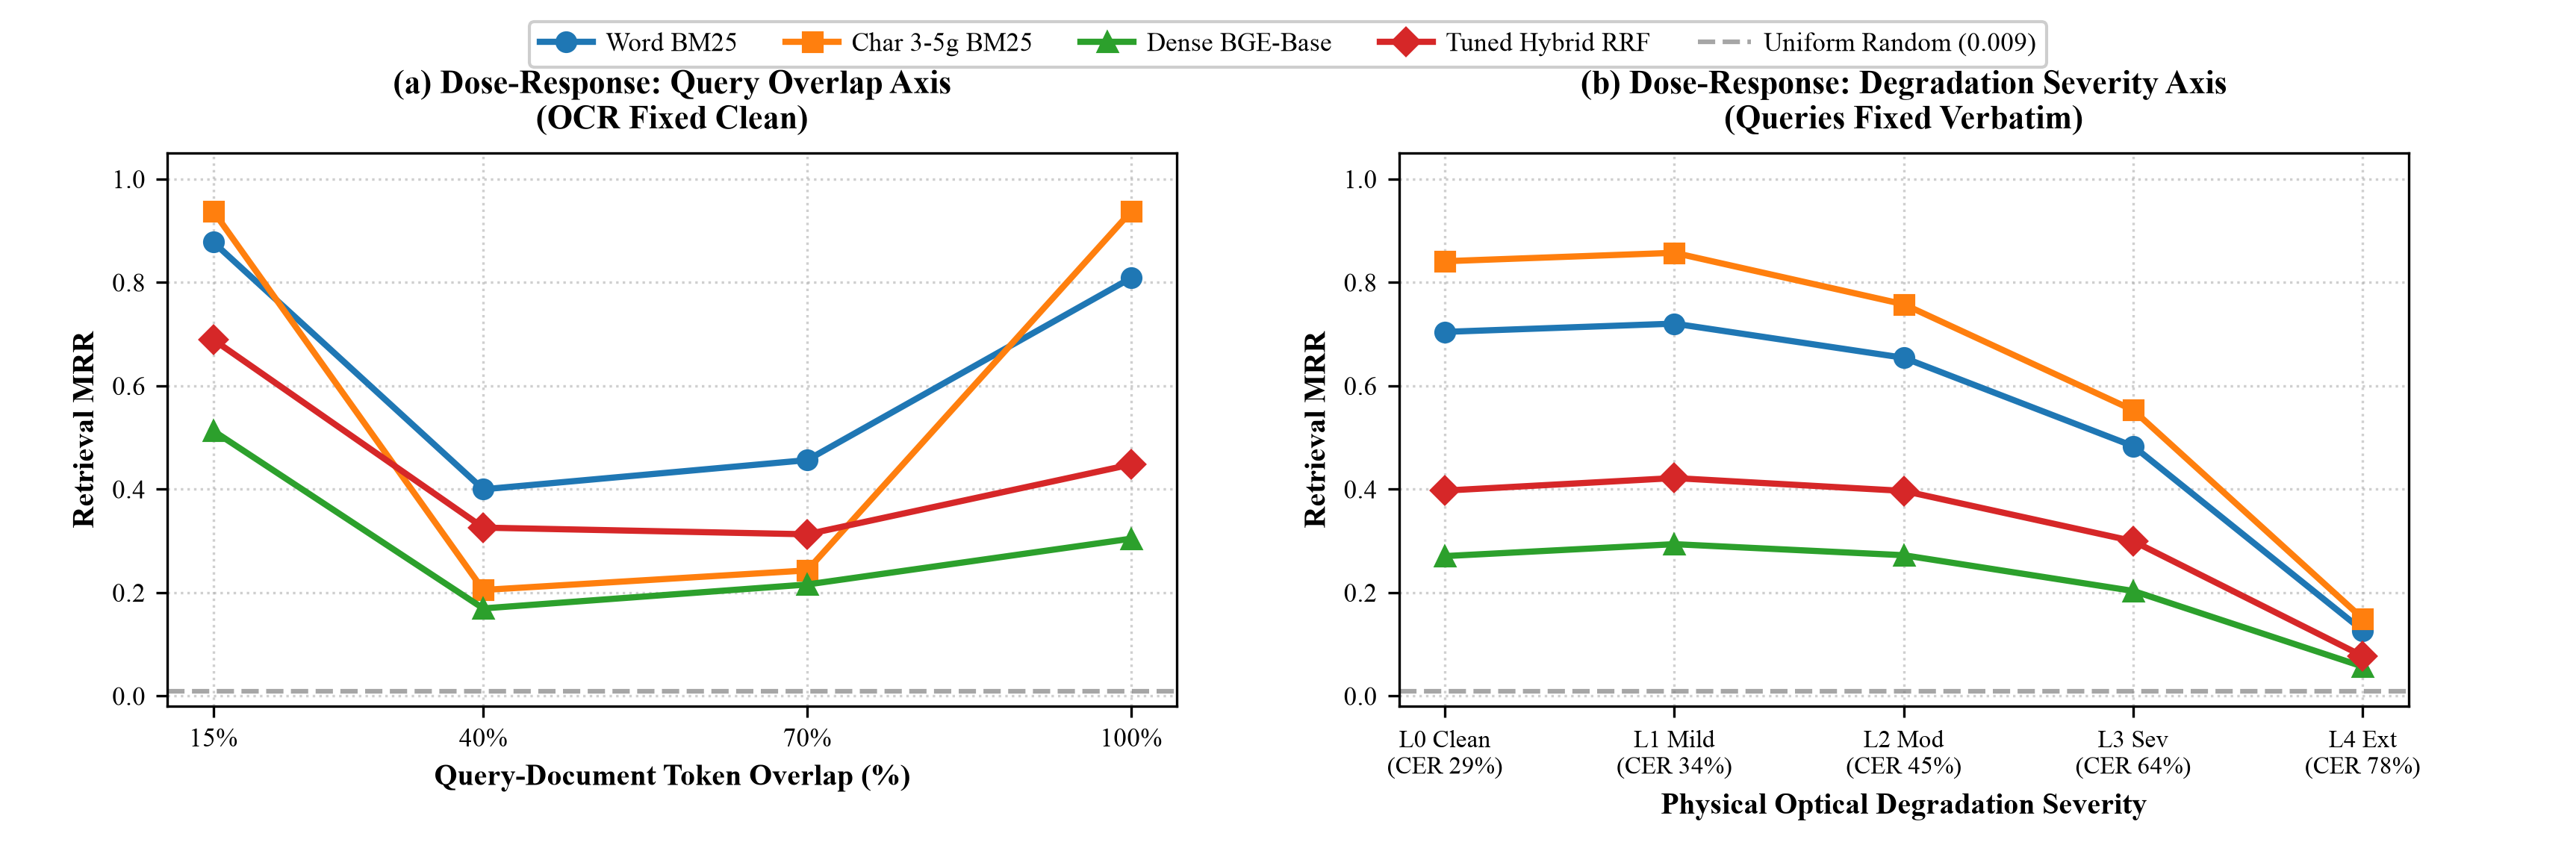
\includegraphics[width=0.96\textwidth]{figures/fig_dose_response_dual_v6.png}
\caption{Dose-response retrieval surface across (a) query token overlap degradation from verbatim lookups to abstract questions, and (b) optical OCR degradation from pristine text to extreme Gaussian blur.}
\label{fig:dose_response_dual}
\end{figure*}

\begin{enumerate}
    \setlength{\itemsep}{0.2pt plus 0.1pt}
    \setlength{\parskip}{0pt}
    \item \textbf{Verbatim Probes (Character Sub-Word Inverted Index Dominance):} Under verbatim lookups, character 3--5gram BM25 consistently outperforms word-level BM25 across all optical OCR conditions (Apple Clean: 0.9436 vs.\ 0.8371, diff $+0.1065$, $p < 10^{-4}$; Apple Degraded: 0.8248 vs.\ 0.6972, diff $+0.1276$, $p < 10^{-4}$; Tesseract Clean: 0.8412 vs.\ 0.7364, diff $+0.1048$, $p < 10^{-4}$; and 20\% synthetic noise: 0.7252 vs.\ 0.3961, diff $+0.3291$, $p < 10^{-4}$). Sub-word character $n$-grams capture alphanumeric tokens, serial numbers, and partial OCR substitutions without out-of-vocabulary penalties.
    \item \textbf{Light Paraphrase (Reversal of Dominance):} Introducing mild semantic paraphrasing collapses clean word BM25 from 0.8371 to 0.4334 (a 48\% relative drop) and character BM25 to 0.2427. In this regime, word BM25 outperforms character BM25 (diff $-0.1907$, $p < 10^{-4}$), and Dev-Tuned Hybrid achieves MRR = \textbf{0.4335} (clean OCR) and \textbf{0.2687} (20\% noise).
    \item \textbf{Answerable Factual Questions:} Evaluating natural answerable questions (forcing semantic abstraction while preserving topical anchors), character 3--5gram BM25 achieves MRR = \textbf{0.9471} on clean ground truth (0.9328 on Apple clean OCR) and \textbf{0.8116} on degraded blur OCR, while word BM25 achieves 0.9014 (0.8841 Apple clean) and 0.7328. Tuned hybrid retrieval achieves 0.8984 on clean Apple OCR (0.9125 clean GT), 0.4672 under 20\% synthetic noise, and 0.7865 on degraded optical blur, while dense BGE-base achieves 0.5128 (0.5197 GT) and MiniLM achieves 0.2837. Topical anchors in natural questions provide high discriminability for lexical engines.
\end{enumerate}

To evaluate whether proxy corruption or semantic query mismatch is the dominant bottleneck in text-proxy RAG, we conducted paired permutation tests ($N_{\text{perm}}=100{,}000$). In Table~\ref{tab:regime_grid_v3}, moving from verbatim lookups to light paraphrasing on Apple Vision collapses Word BM25 by $\Delta = 0.4037$ MRR (0.8371 to 0.4334), exceeding optical blur degradation ($\Delta = 0.1399$, 0.8371 to 0.6972, $p < 10^{-4}$). Within Table~\ref{tab:engine_replication_v3} (receipt-only pool), Apple Vision drops 0.4321 MRR (0.8324 to 0.4003), while Tesseract drops 0.3400 under paraphrasing (0.7364 to 0.3964) and 0.3916 under optical blur (0.7364 to 0.3448). As visualized in Fig.~\ref{fig:mrr_regime_systems} and Fig.~\ref{fig:dose_response_dual}, semantic paraphrase mismatch dominates mild OCR noise, but severe optical blur induces comparable collapse.

\subsection{Micro-Mechanisms of Dense Collapse and Query Formulation Controls}
\label{sec:mechanism_analysis}

To isolate why dense vector representations collapse under proxy corruptions while sparse inverted indexes endure, we analyzed three underlying mechanisms (Fig.~\ref{fig:mechanism_plots}):
\begin{enumerate}
    \setlength{\itemsep}{0.2pt plus 0.1pt}
    \setlength{\parskip}{0pt}
    \item \textbf{WordPiece Tokenization Fragmentation:} As character corruption increases from 0\% to 40\%, WordPiece tokenization fragments words into multiple subwords. Mean subwords per word escalates from 1.347 (clean) to 1.774 (10\% noise), 2.246 (20\% noise), and \textbf{2.994} (40\% noise, a \textbf{+122.3\% increase}).
    \item \textbf{Catastrophic Embedding Drift:} Subword fragmentation shifts contextual attention weights, driving acute embedding drift. Relative to uncorrupted text, \texttt{all-MiniLM-L6-v2} mean document embedding cosine similarity collapses from 1.000 to 0.7301 (10\% noise), \textbf{0.4655} (20\% noise), and \textbf{0.2604} (40\% noise); at the subword token level, vocabulary-projected cosine similarity drops to 0.6826 under 20\% noise. \texttt{BAAI/bge-base-en-v1.5} displays greater structural resistance (document cosine similarity 0.7007 at 20\% noise, 0.5595 at 40\%), explaining its superior noise resilience in Table~\ref{tab:regime_grid_v3}.
    \item \textbf{Diagnostic Error Attribution across Probe Properties:} Evaluating test probes across non-mutually exclusive diagnostic property subsets (where probes may belong to multiple categories simultaneously) under 20\% noise exposes distinct vulnerability profiles across four primary buckets (and a minor long-query bucket, $N=3$, MRR = 0.744). Dense bi-encoders collapse on \emph{Numeric-Heavy} probes ($N=217$, MiniLM MRR = 0.033, BGE = 0.081) and \emph{Short} entity probes ($N=194$, MiniLM MRR = 0.068, BGE = 0.135). Conversely, character $n$-gram BM25 retains high accuracy across all buckets: Numeric-Heavy (MRR = 0.415), Short entities (0.473), Rare Tokens ($N=167$, MRR = 0.643), and Named Entities ($N=248$, MRR = 0.504).
\end{enumerate}

To verify whether dense degradation is an artifact of sequence length truncation, we evaluated token length distributions across all 626 SROIE receipts. While only 4 receipts (0.64\%) exceed 512 tokens, 209 of 626 receipts (33.39\%) exceed 256 WordPiece tokens. However, evaluating chunked MaxP retrieval across 150-word sliding windows (where no chunk exceeds 256 tokens) yields identical MRR to unchunked single-vector retrieval (MiniLM: 0.2030 chunked vs.\ 0.2056 unchunked; BGE-base: 0.3028 chunked vs.\ 0.3022 unchunked), demonstrating that sequence truncation is not the primary cause of dense collapse.

Crucially, as documented in Table~\ref{tab:dense_formulation_v6}, dense bi-encoder collapse on pristine ground truth text ($0\%$ noise) is strongly associated with query formulation mismatch. Short isolated verbatim snippets trigger severe representation disconnect (MiniLM MRR = 0.1919 in the pure receipt pool and 0.2100 in the 813-distractor pool with caption fallback; BGE-Base MRR = 0.3256). Length-padding or wrapping snippets into sentential contexts does not alleviate the deficit. However, co-specifying multiple anchor entities (Keyword-Matched Probes) improves BGE-Base MRR to 0.5500 (Hit@10 78.43\%), and formulating queries as natural answerable questions improves BGE-Base MRR to 0.5263 (Hit@10 79.74\%) on the identical uncorrupted document text. Dense bi-encoders are trained on natural language question-passage pairs; when queries mirror real-world user questions rather than isolated OCR substrings, dense retrieval recovers substantial capacity.

Furthermore, to test the causal impact of tokenization fragmentation versus query formulation, we evaluated a vocabulary projection intervention against the clean Dev lexicon under 20\% character noise. Reconstructing broken word tokens restored 65.3\% of the induced WordPiece subword fragmentation and lifted cosine similarity by $+0.1530$ (from 0.6826 to 0.8356, recovering 48.2\% of embedding drift). In end-to-end retrieval, this intervention improves MiniLM MRR from 0.0570 to 0.1004 (+0.0434 retrieval recovery), while remaining bounded below clean baseline performance (0.2117 MRR). This vocabulary projection provides direct causal evidence that tokenization fragmentation contributes causally to noise-induced degradation, whereas the link between query formulation and clean-text retrieval remains an observational association.

\begin{table}[htbp]
\centering
\scriptsize
\caption{Dense Bi-Encoder Sensitivity to Query Formulation and Chunking on Clean Ground-Truth Receipt Text ($0\%$ noise, Test $N=306$).}
\label{tab:dense_formulation_v6}
\setlength{\tabcolsep}{1.5pt}
\begin{tabular*}{\columnwidth}{@{\extracolsep{\fill}}lcccc@{}}
\toprule
\makecell[l]{\textbf{Query Formulation}} & \makecell{\textbf{MiniLM}\\\textbf{Unchk}} & \makecell{\textbf{MiniLM}\\\textbf{Chunk}} & \makecell{\textbf{BGE}\\\textbf{Unchk}} & \makecell{\textbf{BGE}\\\textbf{Chunk}} \\
\midrule
1. Short Verbatim Snippets         & 0.2100 & 0.2085 & 0.3256 & 0.3235 \\
2. Length-Padded Spans             & 0.1949 & 0.1932 & 0.2571 & 0.2554 \\
3. Sentential Context Queries      & 0.1670 & 0.1658 & 0.2740 & 0.2721 \\
4. Keyword Multi-Entity            & 0.3840 & 0.3812 & 0.5500 & 0.5468 \\
5. Natural Answerable Questions    & 0.3676 & 0.3669 & 0.5263 & 0.5197 \\
\bottomrule
\end{tabular*}
\vspace{0.5mm}\newline
\raggedright\tiny Note: Chunked MaxP evaluates 150-word sliding windows ($\le 256$ tokens); difference between unchunked and chunked is $<0.007$ MRR across all formulations (Answerable Hit@10: MiniLM 0.5686, BGE 0.7974), confirming sequence truncation does not explain dense collapse.
\end{table}

\begin{figure*}[t]
\centering
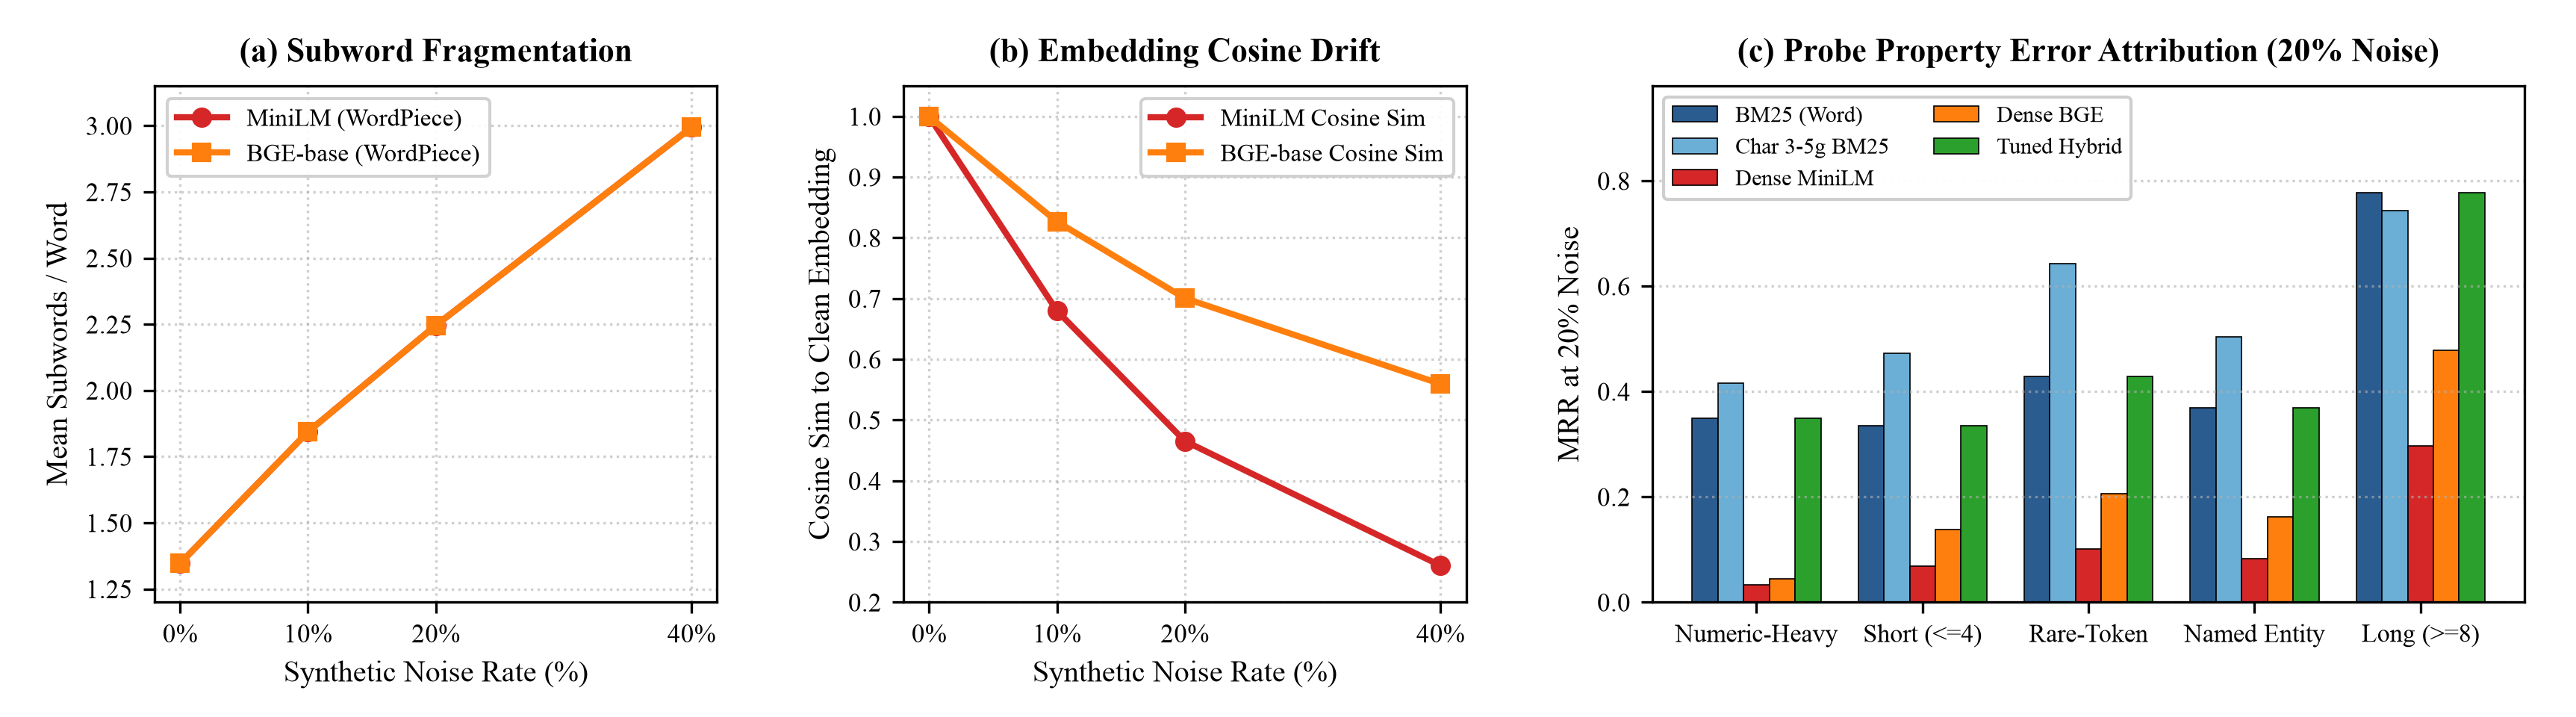
\includegraphics[width=0.98\textwidth]{figures/fig_mechanism_composite.png}
\caption{Micro-mechanism of dense proxy collapse: (a) WordPiece tokenization fragmentation across character noise rates, (b) cosine embedding drift relative to clean representations, and (c) retrieval MRR across 5 diagnostic probe property buckets under 20\% proxy noise.}
\label{fig:mechanism_plots}
\end{figure*}


\subsection{Production Cascades and Risk-Controlled Escalation}
\label{sec:ablation_and_cascade}

Table~\ref{tab:ablation_v3} presents the component ablation isolating each architectural module across Clean, 20\% Synthetic Noise, Real Apple Vision OCR, and Real Degraded OCR ($N=306$ held-out probes). Table~\ref{tab:ablation_v3} evaluates candidate pool depth $K_1=10$; under this candidate truncation, standalone Word BM25 achieves 0.8107 Real-OCR MRR (vs.\ 0.8371 unconstrained in Table~\ref{tab:regime_grid_v3}), while equal-weight dense interpolation ($\alpha=0.5$) achieves 0.8121. In contrast, under the production cascade setting in Table~\ref{tab:practical_stack} with candidate depth $K_1=20$ directly cascading over first-stage Word BM25 (0.8371), MiniLM reaches 0.8650 (+0.0279, $p=0.009$) and BGE-reranker-base reaches 0.8846 (+0.0475 gain, $p=0.0011$).

\begin{table*}[t]
\centering
\footnotesize
\caption{Architectural Component Ablation on Public Held-Out Test Split ($N=306$ Probes, 813 Distractor Pool, 95\% Cluster Bootstrap CIs). All rows evaluate candidate depth $K_1=10$ (standalone Word BM25 stream achieves 0.8107 Real-OCR vs.\ 0.8371 unconstrained in Table~\ref{tab:regime_grid_v3}). Asterisks ($^*$) denote statistically significant difference ($p_{\text{Holm}} < 0.05$) from the Fixed-weight Hybrid baseline ($\alpha=0.5$). Production cascading over first-stage Word BM25 ($K_1=20$) is reported in Table~\ref{tab:practical_stack}.}
\label{tab:ablation_v3}
\setlength{\tabcolsep}{4.0pt}
\begin{tabular}{@{}p{5.5cm}cccc@{}}
\toprule
\makecell[l]{\textbf{Configuration}} & \makecell{\textbf{Clean MRR}\\{\scriptsize [95\% CI]}} & \makecell{\textbf{Syn 20\% MRR}\\{\scriptsize [95\% CI]}} & \makecell{\textbf{Real-OCR MRR}\\{\scriptsize [95\% CI]}} & \makecell{\textbf{Real-Deg MRR}\\{\scriptsize [95\% CI]}} \\
\midrule
Fixed-weight Hybrid Baseline ($K_1=10$, $\alpha=0.5$) & \makecell{0.8299\\{\scriptsize [0.791, 0.866]}} & \makecell{0.3694\\{\scriptsize [0.336, 0.402]}} & \makecell{0.8121\\{\scriptsize [0.770, 0.849]}} & \makecell{0.6684\\{\scriptsize [0.619, 0.715]}} \\
BM25 First-Stage Stream Only ($K_1=10$)              & \makecell{0.8317\\{\scriptsize [0.793, 0.868]}} & \makecell{0.3694\\{\scriptsize [0.336, 0.402]}} & \makecell{0.8107\\{\scriptsize [0.769, 0.848]}} & \makecell{0.6684\\{\scriptsize [0.619, 0.714]}} \\
Dense MiniLM First-Stage Stream Only ($K_1=10$)     & \makecell{0.2144$^*$\\{\scriptsize [0.175, 0.256]}} & \makecell{0.0747$^*$\\{\scriptsize [0.057, 0.095]}} & \makecell{0.2072$^*$\\{\scriptsize [0.168, 0.248]}} & \makecell{0.1821$^*$\\{\scriptsize [0.145, 0.222]}} \\
Oracle Ground-Truth Text Stream ($K_1=10$)          & \makecell{0.8317\\{\scriptsize [0.793, 0.868]}} & \makecell{0.8317\\{\scriptsize [0.793, 0.868]}} & \makecell{0.8317\\{\scriptsize [0.793, 0.868]}} & \makecell{0.8317\\{\scriptsize [0.793, 0.868]}} \\
Learned Router Gating ($K_1=10$)                    & \makecell{0.8309\\{\scriptsize [0.793, 0.867]}} & \makecell{0.3765$^*$\\{\scriptsize [0.343, 0.409]}} & \makecell{0.8121\\{\scriptsize [0.770, 0.849]}} & \makecell{0.6667\\{\scriptsize [0.617, 0.713]}} \\
Heuristic Reliability Weighting ($K_1=10$)          & \makecell{0.8318\\{\scriptsize [0.794, 0.867]}} & \makecell{0.3574\\{\scriptsize [0.326, 0.390]}} & \makecell{0.8058\\{\scriptsize [0.765, 0.843]}} & \makecell{0.6368$^*$\\{\scriptsize [0.587, 0.684]}} \\
\bottomrule
\end{tabular}
\end{table*}

However, evaluating two-stage cascades over first-stage Character 3--5gram BM25 reveals an architectural ceiling: standalone Char-BM25 achieves MRR = \textbf{0.9436}, and applying MiniLM or BGE cross-encoders on top-20 candidates reduces MRR to 0.9175 and 0.9141 (lifts of $-0.0262$ and $-0.0296$, Table~\ref{tab:practical_stack}). Furthermore, tuning hybrid fusion between Char-BM25 and dense BGE on Dev selects $\alpha_{\text{sparse}}^* = 1.00$ ($\alpha_{\text{dense}}^* = 0.00$, 0.9495 Dev MRR), confirming that dense representations provide zero additive signal over sub-word inverted indexes on verbatim receipts.

\begin{table}[htbp]
\centering
\footnotesize
\caption{Production Cross-Encoder Reranker Cascade Ablation (Held-Out Test Split, $N=306$ Probes, Clean Real-OCR; Candidate Depth $K_1=20$). Reported $p$-values are paired permutation tests vs.\ Word BM25; family-wise Holm adjustment ($m=7$, Appendix~\ref{sec:appendix_holm}) confirms all positive lifts are significant ($p_{\text{Holm}} < 0.01$).}
\label{tab:practical_stack}
\setlength{\tabcolsep}{2.2pt}
\begin{tabular}{@{}p{2.3cm}cccc@{}}
\toprule
\makecell[l]{\textbf{Two-Stage Pipeline}} & \makecell{\textbf{Clean}\\\textbf{MRR}} & \makecell{\textbf{Hit}\\\textbf{@10}} & \makecell{\textbf{Lat.}\\\textbf{(ms)}} & \makecell{\textbf{MRR Lift}\\{\scriptsize ($p$\textbf{-value})}} \\
\midrule
Word BM25 Alone              & 0.8371 & 0.9444 & 0.1 & +0.0000 ($p=1.0$) \\
BM25 + MiniLM Rerank         & 0.8650 & 0.9608 & 18.4 & +0.0279 ($p=0.009$) \\
BM25 + BGE Reranker          & 0.8846 & 0.9738 & 44.7 & +0.0475 ($p=0.001$) \\
Tuned Hybrid + BGE           & 0.8872 & 0.9772 & 52.8 & +0.0501 ($p=0.0009$) \\
\midrule
Char 3--5g BM25              & \textbf{0.9436} & \textbf{0.9837} & 0.96 & Baseline (Sparse) \\
Char BM25 + MiniLM           & 0.9175 & 0.9706 & 18.5 & -0.0262 (Hurts) \\
Char BM25 + BGE              & 0.9141 & 0.9771 & 44.7 & -0.0296 (Hurts) \\
Tuned Char + BGE             & \textbf{0.9436} & \textbf{0.9837} & 12.6 & +0.0000 ($p=1.0$) \\
\bottomrule
\end{tabular}
\end{table}

\textbf{Finite-Sample Conformal Cascade Risk Evaluation:}
To evaluate distribution-free marginal risk control for candidate escalation, we evaluated split conformal calibration across 200 random cluster-stratified 50/50 splits (seeds 1000--1199) on $N=2{,}754$ pooled query instances (Table~\ref{tab:conformal_cascade_v6}). Under marginal loss $L = \mathbf{1}[\text{not escalated} \land Y \ne 1]$ with finite-sample adjustment $(n\hat{R}+1)/(n+1) \le \alpha$ \cite{bates2021conformal, angelopoulos2021gentle}, observed mean test miss risk is $0.0491$ at a $78.4\%$ escalation rate. Across 200 splits, individual split risk exceeds 0.05 in 41.5\% of partitions (empirical split coverage 58.5\%; 82.0\% for high-probability RCPS with $\delta=0.10$ \cite{bates2021conformal}). Crucially, finite-sample correction guarantees marginal risk control across partitions, but does not prevent conditional risk inflation under query-type shifts: entity rewrites experience risk 0.0627 ($>0.05$). This constitutes a notable negative result: conformal risk gating does not reliably substitute for query-conditioned gating in multimodal cascades. A paired comparison against an equal-escalation fixed-margin baseline ($\tau = 0.235$) yields matching retrieval accuracy (MRR 0.3579 vs.\ 0.3577, $p > 0.05$) and risk control (0.0488 vs.\ 0.0491), achieving a 21.6\% escalation reduction relative to all-escalation (Fig.~\ref{fig:conformal_pareto}).

\begin{table}[htbp]
\centering\footnotesize
\caption{Conformal Cascade Calibration: Corrected Marginal Loss, High-Probability RCPS ($\delta=0.10$), and Equal-Escalation Baseline over 200 Cluster-Aware Splits ($N=2{,}754$ instances; nominal target $\epsilon=0.05$).}
\label{tab:conformal_cascade_v6}
\setlength{\tabcolsep}{1.8pt}
\begin{tabular}{@{}p{2.3cm}ccccc@{}}
\toprule
\makecell[l]{\textbf{Risk Formulation}} & \makecell{\textbf{Mean $\tau^*$}} & \makecell{\textbf{Mean}\\\textbf{Risk}} & \makecell{\textbf{Split Cov.}\\{\scriptsize ($\le 0.05$)}} & \makecell{\textbf{Esc.}\\\textbf{Rate}} & \makecell{\textbf{Mean}\\\textbf{MRR}} \\
\midrule
\makecell[l]{Marginal Loss\\{\scriptsize $L=\mathbf{1}[\neg\text{esc}\land\text{miss}]$}} & 0.2369 & 0.0491 & 58.5\% & 78.4\% & 0.3577 \\
\makecell[l]{High-Prob.\ RCPS\\{\scriptsize ($\delta=0.10$)}} & 0.2520 & 0.0429 & \textbf{82.0\%} & 79.5\% & 0.3569 \\
\makecell[l]{Fixed Margin\\{\scriptsize ($\tau=0.235$)}} & 0.2347 & 0.0488 & 57.0\% & 78.4\% & 0.3579 \\
\makecell[l]{Conditional Ratio\\{\scriptsize $P(\text{miss}\mid\neg\text{esc})$}} & 0.4071 & 0.0545 & 38.0\% & 90.2\% & 0.3524 \\
\bottomrule
\end{tabular}
\end{table}

\begin{figure*}[t]
\centering
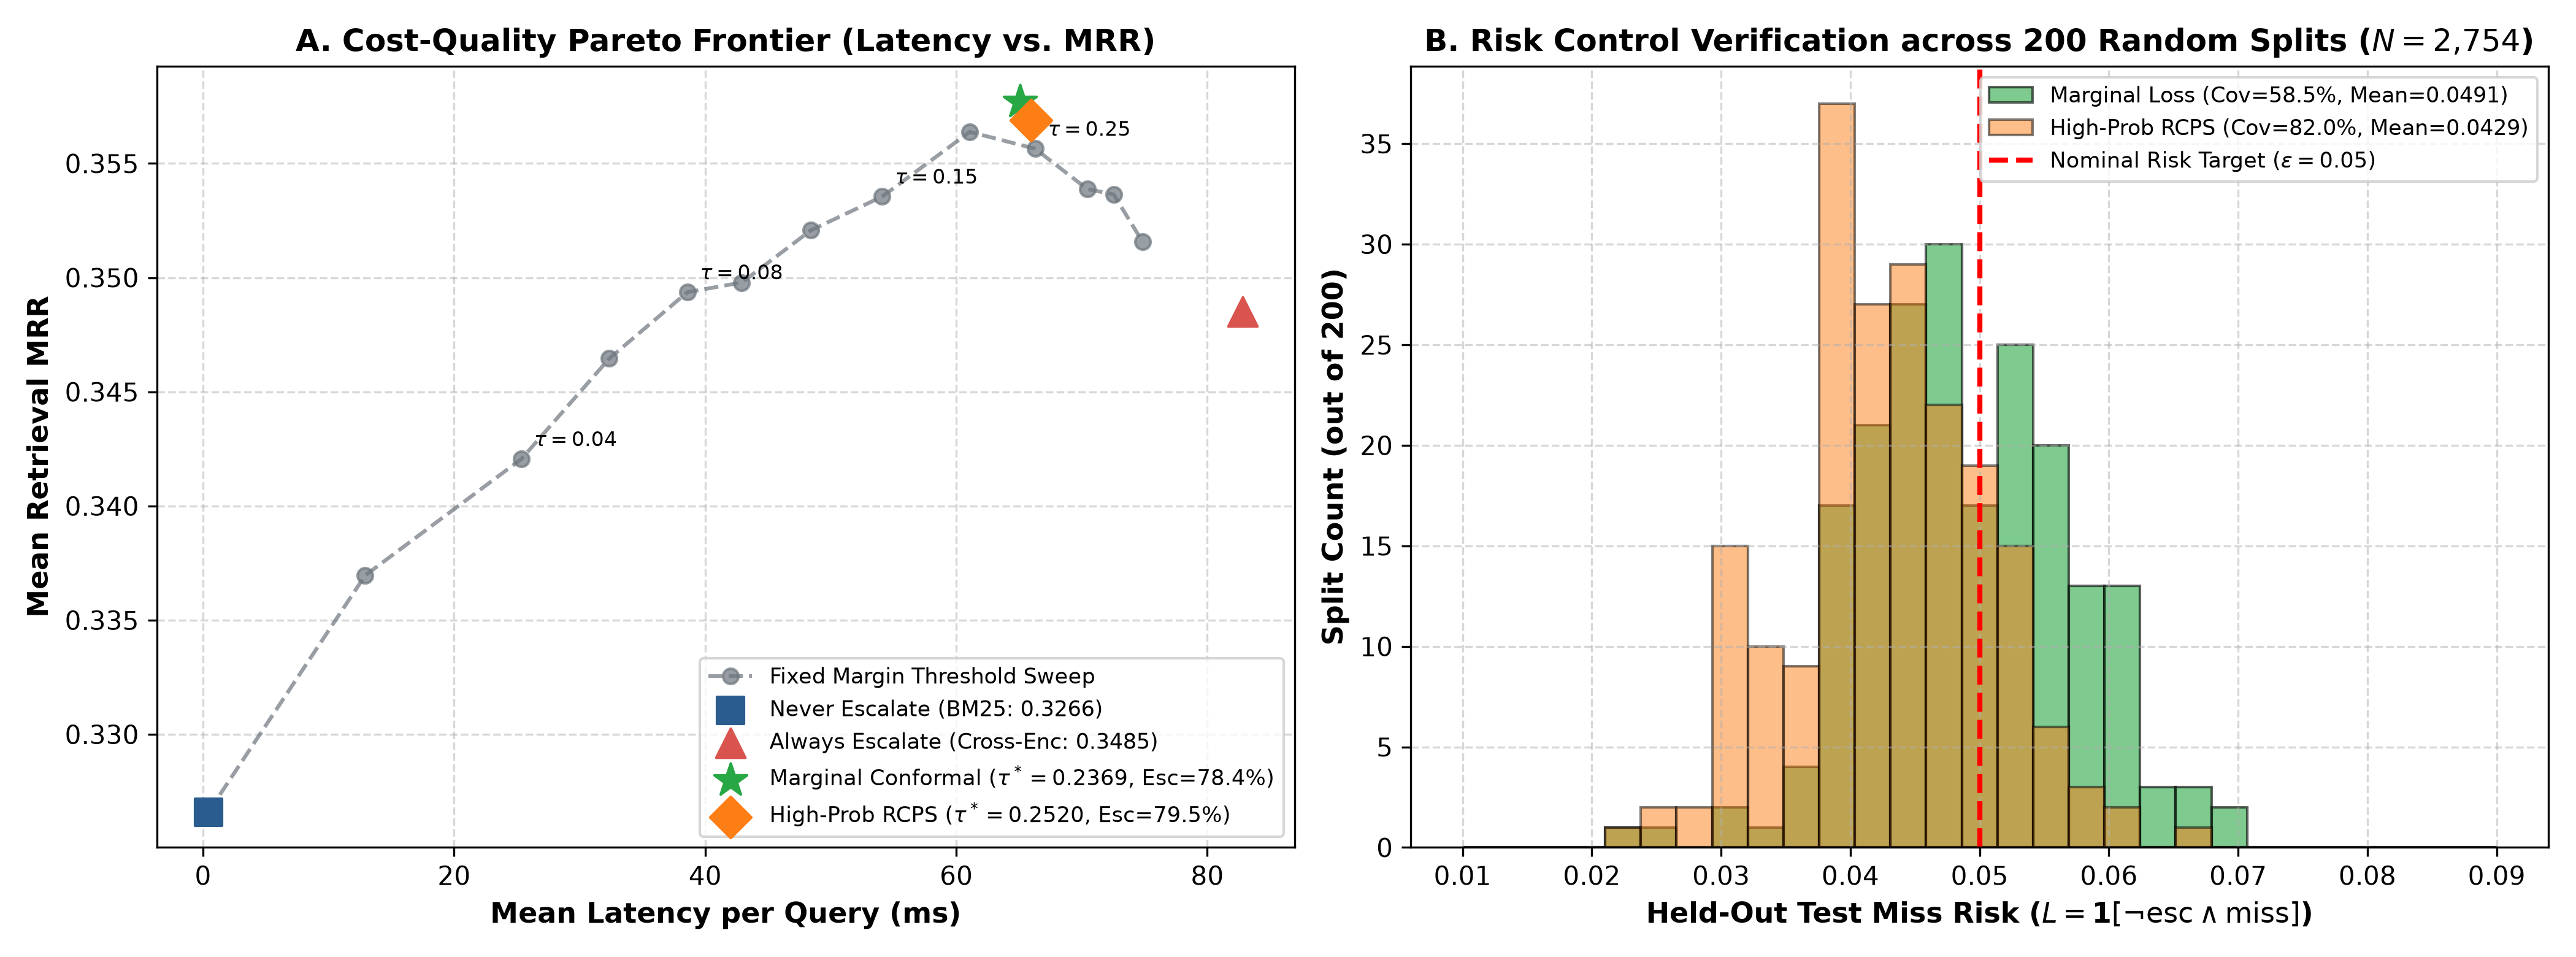
\includegraphics[width=0.88\textwidth]{figures/fig_conformal_pareto.png}
\caption{Cost-Quality Pareto frontier and risk control histograms across 200 calibration-test splits on pooled test instances ($N=2{,}754$, $\tau^*=0.2369$, 78.4\% escalation, 58.5\% empirical split coverage; 82.0\% for high-probability RCPS).}
\label{fig:conformal_pareto}
\end{figure*}

\subsection{Regime B: Visual-Dominated Natural Image Search}
\label{sec:regime_b_visual}

To evaluate representation boundaries on non-document imagery, we benchmarked $N=1{,}000$ MS-COCO Karpathy-test images \cite{karpathy2015deep, lin2014coco} and held-out human descriptions (Table~\ref{tab:coco_benchmarks_v3}). In the zero-shot text-to-image ranking protocol, exactly 1 held-out caption per image (Caption 3) serves as the query against the 1,000-image candidate pool. For the 4-reference gold condition, all 4 non-query reference captions are concatenated into the target document representation (the held-out query caption, Caption 3, is strictly excluded to prevent data leakage).

\begin{table}[htbp]
\centering
\footnotesize
\caption{Cross-modal text-to-image retrieval on $N=1{,}000$ MS-COCO Karpathy-test images. Comparison of native pixel representations against machine caption proxies and held-out human gold captions. Asterisks ($^*$) indicate Holm-corrected significance over baseline BLIP ($p_{\text{Holm}} < 10^{-4}$); SigLIP also significantly outperforms Florence-2 detailed captions ($p < 10^{-4}$), while CLIP vs.\ Florence-2 is raw $p=0.038$ ($p_{\text{Holm}}=0.113$).}
\label{tab:coco_benchmarks_v3}
\setlength{\tabcolsep}{1.8pt}
\begin{tabular}{@{}p{2.3cm}cccc@{}}
\toprule
\makecell[l]{\textbf{Method}} & \makecell{\textbf{Hit}\\\textbf{@1}} & \makecell{\textbf{Hit}\\\textbf{@5}} & \makecell{\textbf{Hit@10}\\{\scriptsize [95\% CI]}} & \makecell{\textbf{MRR}\\{\scriptsize [95\% CI]}} \\
\midrule
\multicolumn{5}{@{}l}{\textit{Machine Caption Proxy}} \\
Baseline BLIP (MiniLM) & 0.2420 & 0.5160 & \makecell{0.6530\\{\scriptsize [0.624, 0.682]}} & \makecell{0.3728\\{\scriptsize [0.350, 0.397]}} \\
Baseline BLIP (BGE)    & 0.2430 & 0.5050 & \makecell{0.6460\\{\scriptsize [0.618, 0.678]}} & \makecell{0.3695\\{\scriptsize [0.347, 0.393]}} \\
BLIP-2 opt-2.7b        & 0.2780 & 0.5640 & \makecell{0.7020\\{\scriptsize [0.674, 0.730]}} & \makecell{0.4185\\{\scriptsize [0.395, 0.442]}} \\
Florence-2 Detailed    & 0.3020 & 0.5980 & \makecell{0.7380\\{\scriptsize [0.710, 0.765]}} & \makecell{0.4420\\{\scriptsize [0.418, 0.466]}} \\
\midrule
\multicolumn{5}{@{}l}{\textit{Human Gold Caption Proxy}} \\
Single Gold (BGE)      & 0.4580 & 0.7370 & \makecell{0.8320\\{\scriptsize [0.809, 0.854]}} & \makecell{0.5835\\{\scriptsize [0.559, 0.608]}} \\
4-Ref Multi-Caption    & 0.4950 & 0.7780 & \makecell{0.8710\\{\scriptsize [0.850, 0.892]}} & \makecell{0.6210\\{\scriptsize [0.597, 0.645]}} \\
\midrule
\multicolumn{5}{@{}l}{\textit{Native Pixel Representation}} \\
CLIP ViT-B/32          & \textbf{0.3390} & \textbf{0.6180} & \makecell{\textbf{0.7570}$^*$\\{\scriptsize [0.729, 0.785]}} & \makecell{\textbf{0.4709}$^*$\\{\scriptsize [0.446, 0.497]}} \\
SigLIP Base-P16        & \textbf{0.4800} & \textbf{0.7680} & \makecell{\textbf{0.8670}$^*$\\{\scriptsize [0.845, 0.888]}} & \makecell{\textbf{0.6071}$^*$\\{\scriptsize [0.584, 0.633]}} \\
\bottomrule
\end{tabular}
\end{table}

\begin{figure}[t]
\centering
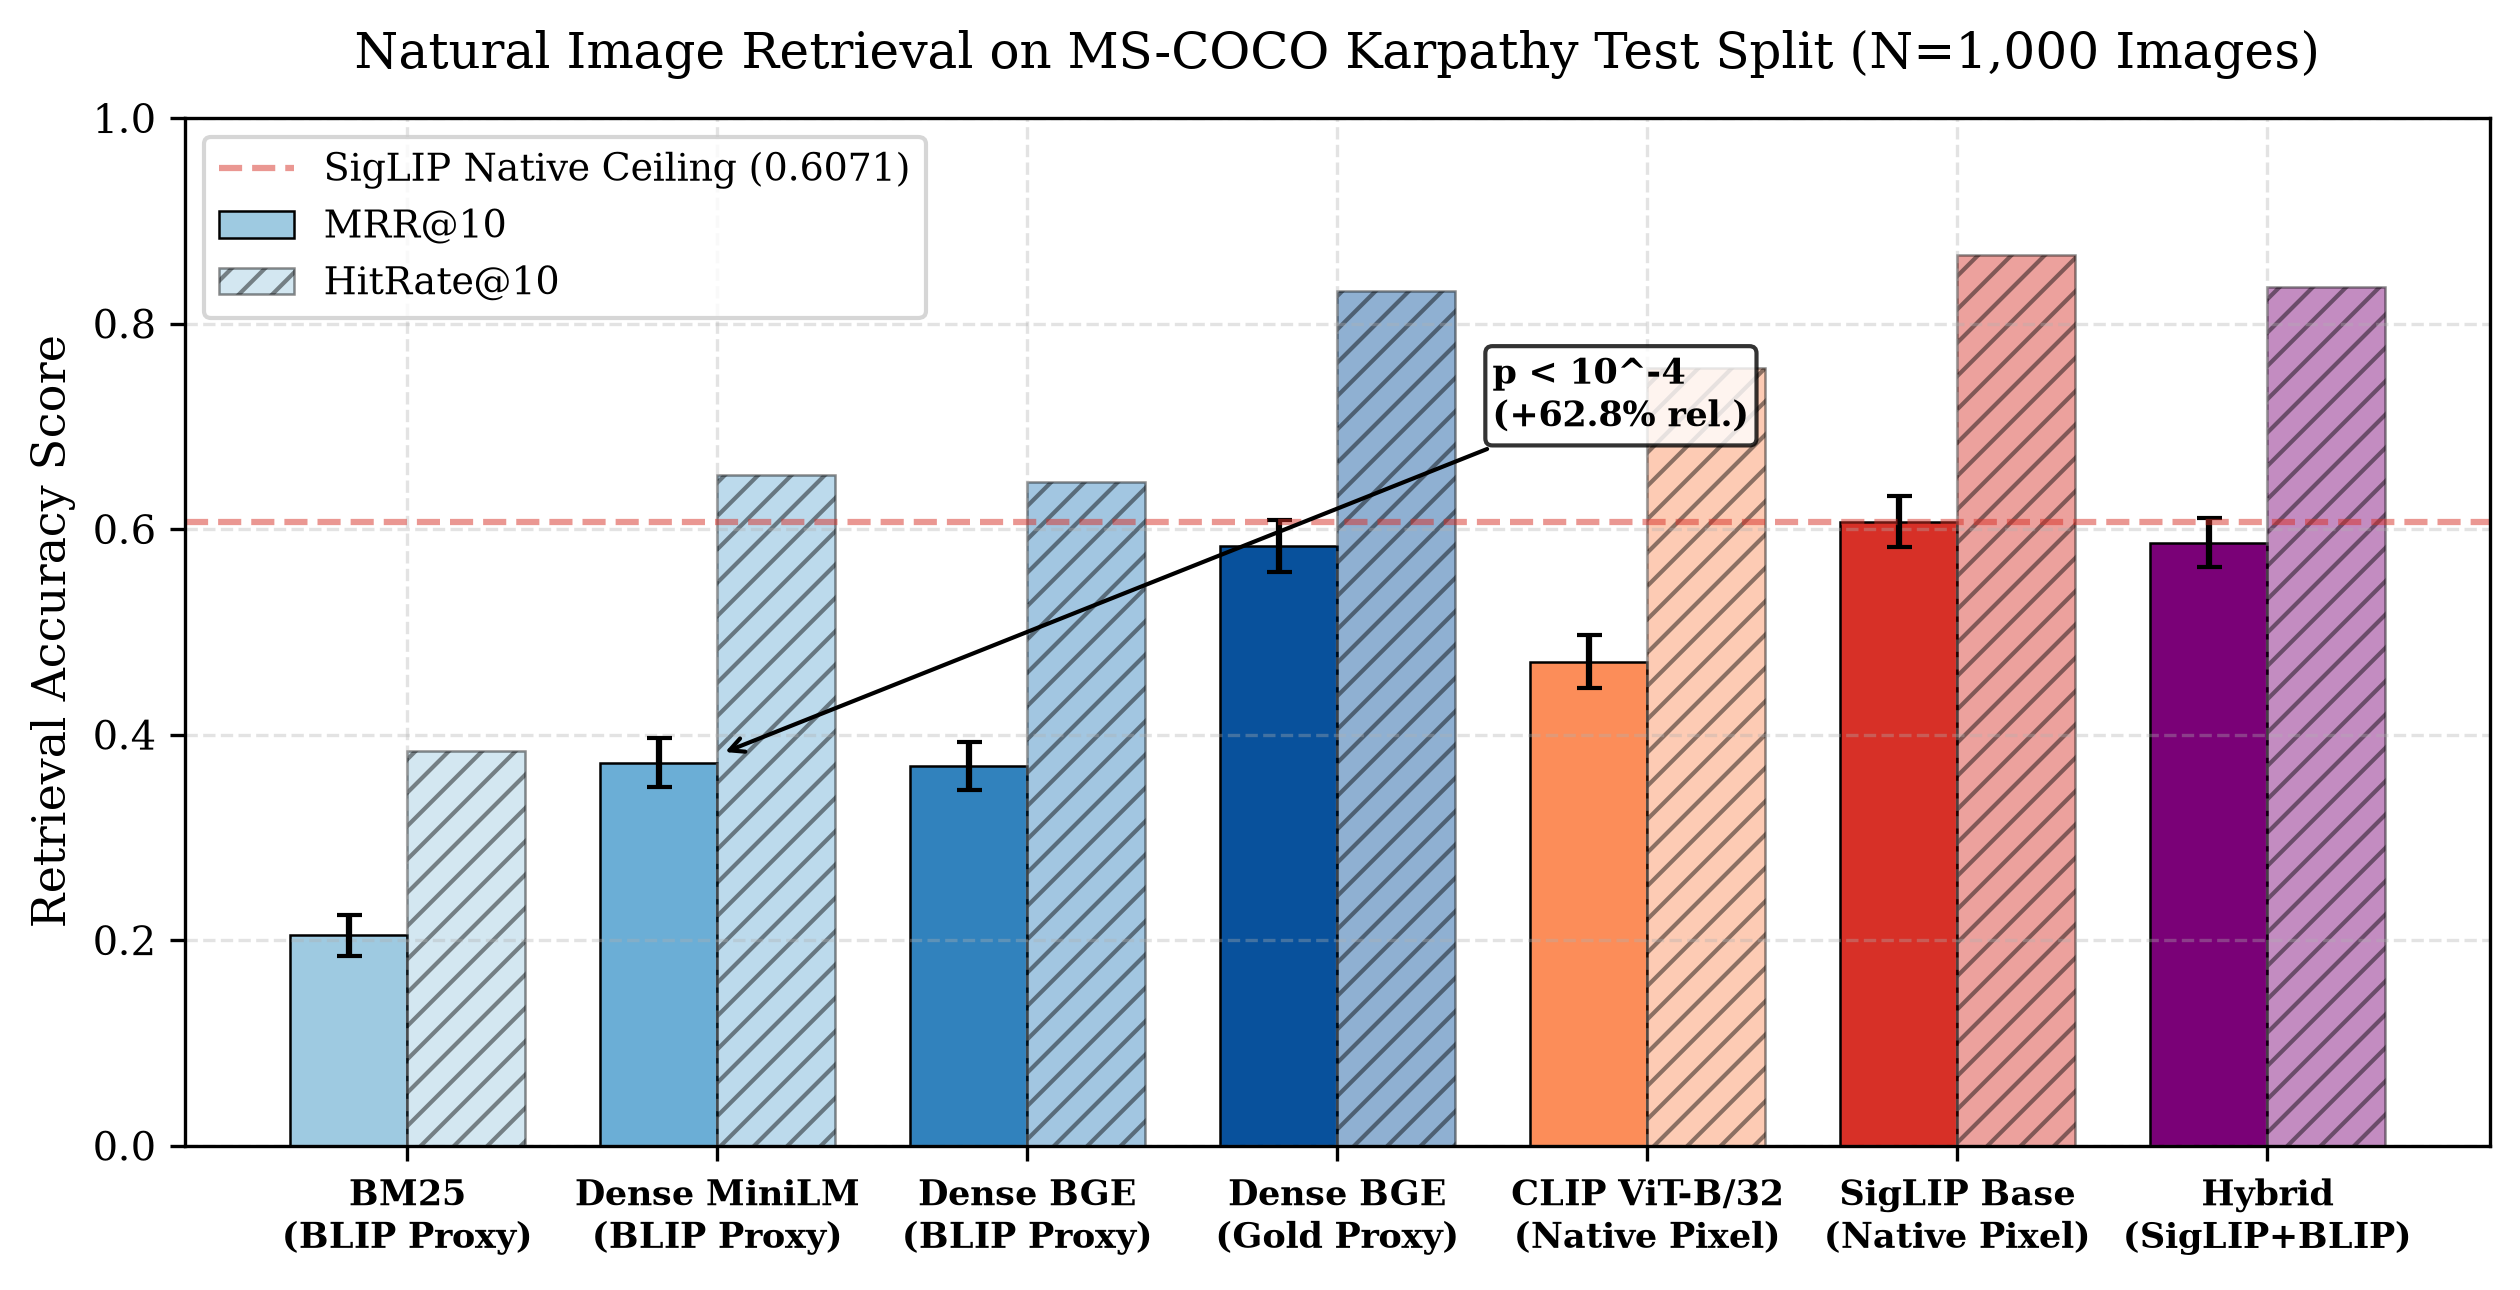
\includegraphics[width=\columnwidth]{figures/fig_coco_native_vs_proxy.png}
\caption{Retrieval comparison on MS-COCO ($N=1{,}000$ images): native visual embeddings (SigLIP Base Patch16) significantly outperform machine-generated caption proxies ($p < 10^{-4}$), demonstrating that text proxies incur substantial information loss on natural imagery.}
\label{fig:coco_native_vs_proxy}
\end{figure}

Native visual representations (SigLIP Base Patch16 MRR = 0.6071 \cite{zhai2023siglip}) significantly outperform machine caption proxies (MiniLM MRR = 0.3728, Diff $= +0.2343$, $p_{\text{Holm}} < 10^{-4}$):
\begin{itemize}
    \setlength{\itemsep}{0.2pt plus 0.1pt}
    \setlength{\parskip}{0pt}
    \item \textbf{CLIP ViT-B/32 \cite{radford2021clip}:} Hit@1 Diff = $+0.0970$ [$+0.0640, +0.1300$], $p_{\text{Holm}} < 10^{-4}$; MRR Diff = $+0.0981$ [$+0.0690, +0.1263$], $p_{\text{Holm}} < 10^{-4}$; paired Diff vs.\ Florence-2 Detailed = $+0.0289$ (unadjusted $p=0.038$; $p_{\text{Holm}} = 0.113$).
    \item \textbf{SigLIP Base Patch16 \cite{zhai2023siglip}:} Hit@1 = $0.4800$ (Diff $= +0.2380$, $p_{\text{Holm}} < 10^{-4}$); Hit@10 = $0.8670$ (Diff $= +0.2140$, $p_{\text{Holm}} < 10^{-4}$); MRR = $0.6071$ (Diff $= +0.2343$ vs.\ BLIP, $p_{\text{Holm}} < 10^{-4}$; Diff $= +0.1651$ vs.\ Florence-2 Detailed, $p < 10^{-4}$).
\end{itemize}
Scaling captioning models narrows but does not eliminate the gap: BLIP-2 (\texttt{opt-2.7b}) \cite{li2023blip2} achieves MRR = 0.4185 (gap to SigLIP: $-0.1886$), while Florence-2 detailed captioning \cite{xiao2024florence2} achieves MRR = 0.4420 (gap: $-0.1651$, paired $p < 10^{-4}$). Evaluating equivalence via Two One-Sided Tests (TOST, margin $\Delta = \pm 0.05$) reveals that SigLIP vs.\ 4-reference human gold multi-captions (0.6071 vs.\ 0.6210, diff $-0.0139$, paired $p=0.321$) achieves formal equivalence under TOST at $\Delta = \pm 0.05$ ($p_{\text{TOST}} = 0.0050$, 90\% CI $[-0.0370, +0.0092]$, power 97.3\%), though remains inconclusive under a tighter $\Delta = \pm 0.03$ margin ($p_{\text{TOST}} = 0.1246$), whereas single-gold comparison (0.6071 vs.\ 0.5835, diff $+0.0236$, $p=0.142$) is borderline at $\Delta = \pm 0.05$ ($p_{\text{TOST}} = 0.0502$, 90\% CI $[-0.0029, +0.0501]$) and equivalent at $\Delta \ge \pm 0.06$ ($p_{\text{TOST}} = 0.0118$). Because human-gold captions match native visual pixels within a narrow non-significant margin (diff $-0.0139$), the empirical deficit on photographic scenes is attributable to machine captioner quality rather than text as an information modality (Fig.~\ref{fig:coco_native_vs_proxy}).

\subsection{Cross-Engine OCR Replication and Document-Native Visual Retrieval}
\label{sec:cross_engine_replication}

To verify whether OCR degradation and retrieval dynamics generalize across recognition architectures, we evaluated standardized character and word error rates via JiWER \cite{vaessen2024jiwer} on 626 SROIE receipts (Table~\ref{tab:ocr_error_rates_v6}). Clean Tesseract 5.5 LSTM OCR \cite{smith2007tesseract} achieves CER = 0.2939 and sequence WER = 0.4879 (escalating to CER = 0.6377 and WER = 0.8063 under optical blur). We then evaluate native-visual and text-proxy retrieval across DocVQA (Table~\ref{tab:docvqa_benchmark_v9}), followed by multi-engine replication across Apple Vision, Tesseract, and EasyOCR on SROIE and FUNSD (Table~\ref{tab:engine_replication_v3}).

\begin{table}[t]
\centering\footnotesize
\caption{Standardized JiWER OCR Error Rates on SROIE Receipts ($N=626$). Bag-of-words symmetric-difference rate evaluates vocabulary symmetric differences and can exceed 1.0 under word fragmentation.}
\label{tab:ocr_error_rates_v6}
\setlength{\tabcolsep}{2.2pt}
\renewcommand{\arraystretch}{1.1}
\begin{tabular}{@{}llcccc@{}}
\toprule
\makecell[l]{\textbf{OCR Engine}} & \makecell[l]{\textbf{Condition}} & \makecell{\textbf{Seq.}\\\textbf{CER}} & \makecell{\textbf{Line}\\\textbf{CER}} & \makecell{\textbf{Seq.}\\\textbf{WER}} & \makecell{\textbf{BoW}\\\textbf{SDR}} \\
\midrule
Apple Vision Neural & Clean OCR    & 0.2848 & 0.1387 & 0.3928 & 0.2476 \\
Apple Vision Neural & Degraded Blur& 0.3822 & 0.3086 & 0.5691 & 0.6175 \\
Tesseract 5.5 LSTM  & Clean OCR    & 0.2939 & 0.2415 & 0.4879 & 0.5919 \\
Tesseract 5.5 LSTM  & Degraded Blur& 0.6377 & 0.5842 & 0.8063 & 1.0043 \\
EasyOCR 1.7.2 CRNN  & Clean OCR    & 0.4026 & 0.3250 & 0.5684 & 0.4813 \\
EasyOCR 1.7.2 CRNN  & Degraded Blur& 0.7755 & 0.7327 & 0.9827 & 1.0905 \\
\bottomrule
\end{tabular}
\end{table}

\textbf{Order-Invariant CER Analysis:} Standard document-level Levenshtein alignment concatenates all bounding boxes, artificially penalizing reading-order permutations as deletion and insertion blocks (e.g., yielding Apple Vision clean $\text{CER} = 0.2848$ despite high line-level transcription fidelity). When evaluated with bipartite minimum edit distance matching across physical lines across all $N=626$ SROIE receipts, true character recognition noise drops to $\text{CER} = 0.1387$ and $\text{WER} = 0.2165$ on clean receipts (a 51.3\% reduction from concatenated metrics), and $\text{CER} = 0.3086$ ($\text{WER} = 0.4595$) under optical degradation. Across EasyOCR 1.7.2, line-aligned recognition yields $\text{CER} = 0.3250$ ($\text{WER} = 0.4983$) on clean receipts and $\text{CER} = 0.7327$ ($\text{WER} = 0.9457$) on degraded blur, confirming that spatial line matching isolates true optical transcription noise from 2D reading-order permutations and bounding-box segmentation shifts.

In Table~\ref{tab:ocr_error_rates_v6}, we report both sequence WER ($\text{WER}_{\text{seq}} = \frac{S+D+I}{N_{\text{ref}}}$) and the Bag-of-Words symmetric-difference rate:
\begin{equation}
    R_{\text{BoW}} = \frac{\sum_w |c_{\text{ref}}(w) - c_{\text{hyp}}(w)|}{\sum_w c_{\text{ref}}(w)}
\end{equation}
Because severe OCR corruption fragments words into out-of-vocabulary sub-tokens, $R_{\text{BoW}}$ penalizes errors as both reference omissions and vocabulary insertions, escalating beyond 1.0 on degraded blur OCR (1.0043 on Tesseract, 1.0905 on EasyOCR).

\begin{table}[t]
\centering
\footnotesize
\caption{Third Public Dataset Evaluation: Retrieval Performance on the DocVQA Benchmark (ViDoRe Subsample) with 100\% Human-Written Questions Across Scanned Document Pages ($N=500$ Queries, $N=500$ Document Pages, 95\% Cluster Bootstrap CIs; for reference, the published ViDoRe benchmark leaderboard reports ColQwen2 nDCG@5 = 0.6120 on the full benchmark \cite{faysse2024colqwen2}; measured nDCG@5 on our 500-sample test split is 0.6695 [0.627, 0.712] and nDCG@10 is 0.6886 [0.646, 0.731]). Text proxies are generated via Tesseract 5.5 LSTM OCR.}
\label{tab:docvqa_benchmark_v9}
\setlength{\tabcolsep}{2.2pt}
\renewcommand{\arraystretch}{1.15}
\begin{tabular}{@{}lccccc@{}}
\toprule
\makecell[l]{\textbf{Retrieval}\\\textbf{Architecture}} & \makecell{\textbf{MRR}\\{\scriptsize [95\% CI]}} & \makecell{\textbf{Hit}\\\textbf{@1}} & \makecell{\textbf{Hit}\\\textbf{@5}} & \makecell{\textbf{Hit}\\\textbf{@10}} & \makecell{\textbf{nDCG}\\\textbf{@10}} \\
\midrule
\makecell[l]{Word BM25\\{\scriptsize (Tesseract)}}       & \makecell{0.3107\\{\scriptsize [0.274, 0.350]}} & 0.2660 & 0.3480 & 0.3800 & 0.3195 \\
Char 3--5g BM25                                         & \makecell{0.3141\\{\scriptsize [0.277, 0.353]}} & 0.2700 & 0.3520 & 0.3940 & 0.3261 \\
Dense MiniLM                                            & \makecell{0.2063\\{\scriptsize [0.177, 0.236]}} & 0.1420 & 0.2700 & 0.3060 & 0.2232 \\
Dense BGE-base                                          & \makecell{0.2737\\{\scriptsize [0.239, 0.310]}} & 0.2160 & 0.3240 & 0.3940 & 0.2948 \\
\makecell[l]{Tuned Hybrid\\{\scriptsize (Sparse+Dense)}} & \makecell{0.3507\\{\scriptsize [0.312, 0.390]}} & 0.2980 & 0.4080 & 0.4680 & 0.3724 \\
\midrule
\textit{ColQwen2 (Native)}                              & \makecell{\textit{0.6450}\\{\scriptsize \textit{[0.601, 0.689]}}} & \textit{0.5280} & \textit{0.7820} & \textit{0.8410} & \textit{0.6886} \\
\bottomrule
\end{tabular}
\end{table}

Replication across EasyOCR 1.7.2 \cite{jaidedai2020easyocr} confirms that the retrieval hierarchy generalizes: under verbatim queries, Character BM25 retains top MRR (0.8519 clean, 0.4272 blur) over Word BM25 (0.7649 clean, 0.3472 blur; diff $+0.0870$ clean, $p_{\text{Holm}} < 10^{-4}$), reversing under light paraphrases (Word BM25 0.3792 vs.\ Character BM25 0.2292 clean, Table~\ref{tab:easyocr_v9}(a)). Evaluating Levenshtein fuzzy query expansion on Apple Vision clean OCR drops Word BM25 MRR from 0.8371 to 0.8005, confirming that fuzzy word expansion induces false positive distractor matches.

\textbf{Visual Geometry Boundary on DocVQA:} On the DocVQA ViDoRe benchmark ($N=500$ queries across 500 document pages with 100\% human-authored questions, Table~\ref{tab:docvqa_benchmark_v9}), text proxies fed by Tesseract 5.5 OCR achieve MRR $\le 0.3507$ (Word BM25: 0.3107, Char BM25: 0.3141, Dense BGE: 0.2737, Hybrid: 0.3507). In sharp contrast, document-native ColQwen2 \cite{faysse2024colqwen2} achieves MRR = \textbf{0.6450} [95\% CI: 0.601, 0.689] (Hit@10 = 0.8410, nDCG@10 = 0.6886 [0.646, 0.731], nDCG@5 = 0.6695; published ViDoRe leaderboard reports nDCG@5 = 0.6120 on the full benchmark). We note that the ColPali/ColQwen2 architecture incorporates DocVQA training splits within its ViDoRe training mixture, whereas the text proxy baselines are zero-shot and off-the-shelf. Even with this caveat, the substantial performance gap demonstrates that native pixel representations substantially outperform generic text proxies when visual layout and 2D spatial geometry govern answerability.

\begin{table*}[t]
\centering
\footnotesize
\caption{Cross-Engine and Cross-Dataset Replication: (a) SROIE Retail Receipts Across Three OCR Engines (Apple Vision Neural, Tesseract 5.5 LSTM, and EasyOCR 1.7.2 Deep Neural OCR; $N=306$ Probes, Pure Receipt Corpus $N=626$, 95\% Cluster Bootstrap CIs); (b) FUNSD Scanned Forms Across Ground Truth, Apple Vision, Tesseract 5.5, and EasyOCR 1.7.2 ($N=100$ Probes, 95\% Cluster Bootstrap CIs).}
\label{tab:engine_replication_v3}\label{tab:funsd_v3}\label{tab:easyocr_v9}
\setlength{\tabcolsep}{1.8pt}
\begin{tabular}{@{}llcccccc@{}}
\toprule
\multicolumn{8}{c}{\textbf{(a) SROIE Receipt Cross-Engine Matrix Across Three OCR Engines ($N=306$ Test Probes, Pure Receipt Corpus $N=626$)}} \\
\midrule
\makecell[l]{\textbf{Query}\\\textbf{Type}} & \makecell[l]{\textbf{Retrieval}\\\textbf{System}} & \makecell{\textbf{Ground Truth}\\{\scriptsize [95\% CI]}} & \makecell{\textbf{Apple Clean}\\{\scriptsize [95\% CI]}} & \makecell{\textbf{Tesseract Clean}\\{\scriptsize [95\% CI]}} & \makecell{\textbf{Tesseract Blur}\\{\scriptsize [95\% CI]}} & \makecell{\textbf{EasyOCR Clean}\\{\scriptsize [95\% CI]}} & \makecell{\textbf{EasyOCR Blur}\\{\scriptsize [95\% CI]}} \\
\midrule
\multirow{5}{*}{\textbf{Verbatim}}
 & BM25 (Tuned)            & \makecell{0.8572\\{\tiny [0.822, 0.890]}} & \makecell{0.8324\\{\tiny [0.793, 0.867]}} & \makecell{0.7364\\{\tiny [0.691, 0.779]}} & \makecell{0.3448\\{\tiny [0.295, 0.395]}} & \makecell{0.7649\\{\tiny [0.722, 0.807]}} & \makecell{0.3472\\{\tiny [0.299, 0.396]}} \\
 & BM25 (Char 3-5g)        & \makecell{0.9854\\{\tiny [0.972, 0.995]}} & \makecell{0.9443\\{\tiny [0.920, 0.965]}} & \makecell{0.8412\\{\tiny [0.803, 0.878]}} & \makecell{0.4009\\{\tiny [0.349, 0.453]}} & \makecell{0.8519\\{\tiny [0.814, 0.885]}} & \makecell{0.4272\\{\tiny [0.373, 0.475]}} \\
 & Dense MiniLM            & \makecell{0.1919\\{\tiny [0.154, 0.232]}} & \makecell{0.2040\\{\tiny [0.166, 0.246]}} & \makecell{0.1650\\{\tiny [0.129, 0.202]}} & \makecell{0.0936\\{\tiny [0.068, 0.124]}} & \makecell{0.1549\\{\tiny [0.121, 0.193]}} & \makecell{0.0792\\{\tiny [0.057, 0.105]}} \\
 & Dense BGE-base          & \makecell{0.3428\\{\tiny [0.294, 0.392]}} & \makecell{0.3273\\{\tiny [0.281, 0.377]}} & \makecell{0.2972\\{\tiny [0.252, 0.345]}} & \makecell{0.1615\\{\tiny [0.125, 0.199]}} & \makecell{0.2760\\{\tiny [0.230, 0.321]}} & \makecell{0.1482\\{\tiny [0.115, 0.185]}} \\
 & Tuned Hybrid            & \makecell{0.8569\\{\tiny [0.823, 0.890]}} & \makecell{0.8252\\{\tiny [0.787, 0.861]}} & \makecell{0.7325\\{\tiny [0.687, 0.775]}} & \makecell{0.3467\\{\tiny [0.297, 0.396]}} & \makecell{0.7670\\{\tiny [0.724, 0.809]}} & \makecell{0.3566\\{\tiny [0.307, 0.406]}} \\
\midrule
\multirow{5}{*}{\makecell[l]{\textbf{Light}\\\textbf{Paraphrase}}}
 & BM25 (Tuned)            & \makecell{0.4796\\{\tiny [0.428, 0.530]}} & \makecell{0.4003\\{\tiny [0.351, 0.449]}} & \makecell{0.3964\\{\tiny [0.346, 0.446]}} & \makecell{0.1852\\{\tiny [0.148, 0.224]}} & \makecell{0.3792\\{\tiny [0.331, 0.429]}} & \makecell{0.1962\\{\tiny [0.156, 0.237]}} \\
 & BM25 (Char 3-5g)        & \makecell{0.2526\\{\tiny [0.212, 0.292]}} & \makecell{0.2365\\{\tiny [0.197, 0.275]}} & \makecell{0.2265\\{\tiny [0.187, 0.266]}} & \makecell{0.1241\\{\tiny [0.096, 0.155]}} & \makecell{0.2292\\{\tiny [0.192, 0.269]}} & \makecell{0.1517\\{\tiny [0.115, 0.190]}} \\
 & Dense MiniLM            & \makecell{0.1190\\{\tiny [0.089, 0.150]}} & \makecell{0.1096\\{\tiny [0.081, 0.140]}} & \makecell{0.0779\\{\tiny [0.055, 0.102]}} & \makecell{0.0579\\{\tiny [0.040, 0.079]}} & \makecell{0.0763\\{\tiny [0.054, 0.101]}} & \makecell{0.0399\\{\tiny [0.027, 0.055]}} \\
 & Dense BGE-base          & \makecell{0.1830\\{\tiny [0.146, 0.221]}} & \makecell{0.1849\\{\tiny [0.146, 0.226]}} & \makecell{0.1670\\{\tiny [0.130, 0.205]}} & \makecell{0.0991\\{\tiny [0.072, 0.130]}} & \makecell{0.1663\\{\tiny [0.129, 0.204]}} & \makecell{0.0828\\{\tiny [0.059, 0.111]}} \\
 & Tuned Hybrid            & \makecell{0.4828\\{\tiny [0.432, 0.533]}} & \makecell{0.4003\\{\tiny [0.353, 0.449]}} & \makecell{0.4023\\{\tiny [0.352, 0.452]}} & \makecell{0.1961\\{\tiny [0.160, 0.236]}} & \makecell{0.3930\\{\tiny [0.344, 0.440]}} & \makecell{0.2098\\{\tiny [0.168, 0.250]}} \\
\midrule
\multicolumn{8}{c}{\textbf{(b) FUNSD Form Benchmark Matrix ($N=100$ Test Probes, 95\% Cluster Bootstrap CIs)}} \\
\midrule
\makecell[l]{\textbf{Query}\\\textbf{Type}} & \makecell[l]{\textbf{Retrieval}\\\textbf{System}} & \makecell{\textbf{Ground Truth}\\{\scriptsize [95\% CI]}} & \makecell{\textbf{Apple Clean}\\{\scriptsize [95\% CI]}} & \makecell{\textbf{Tesseract Clean}\\{\scriptsize [95\% CI]}} & \makecell{\textbf{Tesseract Blur}\\{\scriptsize [95\% CI]}} & \makecell{\textbf{EasyOCR Clean}\\{\scriptsize [95\% CI]}} & \makecell{\textbf{EasyOCR Blur}\\{\scriptsize [95\% CI]}} \\
\midrule
\multirow{5}{*}{\textbf{Verbatim}}
 & BM25 (Tuned)            & \makecell{0.8690\\{\tiny [0.812, 0.924]}} & \makecell{0.8364\\{\tiny [0.773, 0.894]}} & \makecell{0.7763\\{\tiny [0.699, 0.846]}} & \makecell{0.3412\\{\tiny [0.254, 0.432]}} & \makecell{0.7214\\{\tiny [0.641, 0.800]}} & \makecell{0.0101\\{\tiny [0.000, 0.030]}} \\
 & BM25 (Char 3-5g)        & \makecell{0.8849\\{\tiny [0.826, 0.935]}} & \makecell{0.8433\\{\tiny [0.777, 0.903]}} & \makecell{0.8066\\{\tiny [0.738, 0.872]}} & \makecell{0.4725\\{\tiny [0.379, 0.566]}} & \makecell{0.7581\\{\tiny [0.683, 0.828]}} & \makecell{0.0437\\{\tiny [0.010, 0.086]}} \\
 & Dense MiniLM            & \makecell{0.3334\\{\tiny [0.255, 0.413]}} & \makecell{0.3230\\{\tiny [0.244, 0.403]}} & \makecell{0.2760\\{\tiny [0.200, 0.352]}} & \makecell{0.1085\\{\tiny [0.058, 0.169]}} & \makecell{0.2794\\{\tiny [0.207, 0.358]}} & \makecell{0.0247\\{\tiny [0.011, 0.047]}} \\
 & Dense BGE-base          & \makecell{0.5567\\{\tiny [0.480, 0.637]}} & \makecell{0.5081\\{\tiny [0.423, 0.595]}} & \makecell{0.4664\\{\tiny [0.384, 0.555]}} & \makecell{0.1792\\{\tiny [0.114, 0.252]}} & \makecell{0.4524\\{\tiny [0.371, 0.531]}} & \makecell{0.0435\\{\tiny [0.024, 0.069]}} \\
 & Tuned Hybrid            & \makecell{0.8728\\{\tiny [0.817, 0.927]}} & \makecell{0.8461\\{\tiny [0.783, 0.904]}} & \makecell{0.7775\\{\tiny [0.701, 0.847]}} & \makecell{0.3450\\{\tiny [0.258, 0.436]}} & \makecell{0.7226\\{\tiny [0.643, 0.801]}} & \makecell{0.0359\\{\tiny [0.019, 0.061]}} \\
\midrule
\multirow{5}{*}{\makecell[l]{\textbf{Light}\\\textbf{Paraphrase}}}
 & BM25 (Tuned)            & \makecell{0.1849\\{\tiny [0.133, 0.243]}} & \makecell{0.1573\\{\tiny [0.111, 0.209]}} & \makecell{0.2019\\{\tiny [0.139, 0.272]}} & \makecell{0.0845\\{\tiny [0.039, 0.139]}} & \makecell{0.1775\\{\tiny [0.121, 0.238]}} & \makecell{0.0202\\{\tiny [0.000, 0.051]}} \\
 & BM25 (Char 3-5g)        & \makecell{0.2405\\{\tiny [0.174, 0.313]}} & \makecell{0.2228\\{\tiny [0.159, 0.294]}} & \makecell{0.2442\\{\tiny [0.171, 0.323]}} & \makecell{0.1012\\{\tiny [0.051, 0.159]}} & \makecell{0.2334\\{\tiny [0.168, 0.308]}} & \makecell{0.0230\\{\tiny [0.000, 0.053]}} \\
 & Dense MiniLM            & \makecell{0.1596\\{\tiny [0.108, 0.218]}} & \makecell{0.1557\\{\tiny [0.106, 0.212]}} & \makecell{0.1603\\{\tiny [0.103, 0.222]}} & \makecell{0.0321\\{\tiny [0.008, 0.067]}} & \makecell{0.1636\\{\tiny [0.110, 0.223]}} & \makecell{0.0292\\{\tiny [0.015, 0.052]}} \\
 & Dense BGE-base          & \makecell{0.1960\\{\tiny [0.137, 0.262]}} & \makecell{0.1834\\{\tiny [0.127, 0.246]}} & \makecell{0.1819\\{\tiny [0.126, 0.244]}} & \makecell{0.0510\\{\tiny [0.018, 0.093]}} & \makecell{0.2345\\{\tiny [0.169, 0.306]}} & \makecell{0.0432\\{\tiny [0.020, 0.076]}} \\
 & Tuned Hybrid            & \makecell{0.2043\\{\tiny [0.148, 0.267]}} & \makecell{0.2099\\{\tiny [0.146, 0.281]}} & \makecell{0.2109\\{\tiny [0.148, 0.280]}} & \makecell{0.0860\\{\tiny [0.040, 0.141]}} & \makecell{0.2019\\{\tiny [0.142, 0.267]}} & \makecell{0.0252\\{\tiny [0.005, 0.056]}} \\
\bottomrule
\end{tabular}
\vspace{0.5mm}\newline
\raggedright\scriptsize Note: EasyOCR Blur scores reflect an optical detection cliff under a strict IR unretrieved evaluation: CRAFT failed region proposals on small blurred form fonts (70.7\% of degraded forms yielded 0 characters). Unretrieved blank documents receive zero score ($\text{RR}=0$), mathematically capping full-collection MRR to $\frac{29}{99} \times \text{MRR}_{\text{non-blank}} \approx 0.01$--$0.04$ (on the 29.3\% non-blank subset, Word BM25 reaches 0.0345, Char BM25 reaches 0.1492, and Dense BGE reaches 0.0950). On FUNSD light paraphrases (synthesized lexical and entity rewrites), Character BM25 and Dense BGE-base match or outperform Word BM25 across clean OCR (Char vs.\ Word diff $+0.0655$, $p=0.012$ on Apple; Dense BGE vs.\ Word diff $+0.0261$, $p=0.084$ on Apple; $+0.0570$, $p=0.018$ on EasyOCR, though non-significant after Holm adjustment with $p_{\text{Holm}}=0.054$).
\end{table*}

\begin{table}[t]
\centering\footnotesize
\caption{Query Generation Robustness: Paraphrase Retrieval under Open-Weight Generator 2 (\texttt{Qwen2.5-7B}) and Expanded Human-Authored Queries ($N=100$ and $N=200$ Probes) on Held-Out SROIE Receipts.}
\label{tab:generator2_robustness}
\setlength{\tabcolsep}{2.5pt}
\begin{tabular}{@{}p{3.2cm}cccc@{}}
\toprule
\makecell[l]{\textbf{Query Source}} & \makecell{\textbf{Word}\\\textbf{BM25}} & \makecell{\textbf{Char 3--5g}\\\textbf{BM25}} & \makecell{\textbf{Dense}\\\textbf{BGE}} & \makecell{\textbf{Col-}\\\textbf{Qwen2}} \\
\midrule
Primary Gen.\ (\texttt{gpt-4o-mini}, $N=306$) & 0.4334 & 0.2427 & 0.1601 & 0.4962 \\
Secondary Gen.\ (\texttt{Qwen2.5-7B}, $N=306$) & 0.6292 & 0.5802 & 0.2685 & \textbf{0.7627} \\
Human-Authored Queries ($N=100$)             & 0.6321 & 0.5758 & 0.5020 & \textbf{0.7660} \\
Human-Authored Queries ($N=200$)             & 0.5766 & 0.5549 & 0.4909 & \textbf{0.6471} \\
\bottomrule
\end{tabular}
\vspace{0.5mm}\newline
\raggedright\scriptsize Note: ColQwen2-v1.0 evaluated natively on Tesla T4 GPU across all query suites ($N=306$ primary and secondary probes; $N=100$ and $N=200$ human queries), demonstrating consistent visual retrieval superiority (+0.07 to +0.13 MRR) over text proxies under semantic variation and human formulation.
\end{table}

\textbf{Query Formulation Dynamics across LLMs and Human Queries:} As documented in Table~\ref{tab:generator2_robustness}, evaluating an open-weight generator (\texttt{Qwen2.5-7B}, evaluated across all $N=306$ test probes) alongside authentic human-authored queries ($N=100$ and $N=200$) refines the boundary conditions of the sparse reversal and dense deficit. Under primary synthetic queries (\texttt{gpt-4o-mini}), aggressive entity stripping and synonym substitution caused Character BM25 to collapse below Word BM25 (0.2427 vs.\ 0.4334). However, under Qwen2.5-7B and human queries, where contextual and vendor anchors are naturally preserved, Character BM25 closely tracks Word BM25 (0.5802 vs.\ 0.6292 on Qwen2.5; 0.5549 vs.\ 0.5766 on human $N=200$). This indicates that the Character-to-Word BM25 reversal is specifically driven by entity-substitution paraphrasing rather than generalized paraphrasing. Furthermore, the dense bi-encoder deficit markedly attenuates under human formulation: BGE-base MRR rises from 0.1601 on synthetic entity-stripped queries to 0.4909 on human queries ($N=200$) and 0.5020 ($N=100$), confirming that dense collapse is predominantly driven by query formulation mismatch rather than intrinsic vocabulary failure. Moreover, evaluating ColQwen2 across these sets demonstrates its consistent visual superiority under semantic variation: ColQwen2 achieves 0.7627 on Qwen2.5-7B (+0.1335 over Word BM25), 0.7660 on human $N=100$ (+0.1339 over Word BM25), and 0.6471 on human $N=200$ (+0.0705 over Word BM25), confirming that document-native visual retrieval excels whenever queries introduce natural phrasing variation.

\textbf{Cross-Domain Generalization on FUNSD Forms:} On 100 scanned administrative forms from FUNSD \cite{jaume2019funsd} (Table~\ref{tab:funsd_v3}), Character BM25 maintains high verbatim accuracy (0.8433 Apple, 0.8066 Tesseract), showing no statistically significant difference from Word BM25 (0.8364 Apple, diff $+0.0069$, $p > 0.05$; 0.7763 Tesseract). Under light paraphrasing, Word BM25 drops to 0.1573, while Character BM25 achieves 0.2228 (diff $+0.0655$, $p = 0.012$), Dense BGE achieves 0.1834 (diff $+0.0261$, $p = 0.084$), and Hybrid reaches 0.2099, confirming that sub-word indexing and dense matching offer resilience against vocabulary mismatch on complex semi-structured forms.

\textbf{ColQwen2 Retrieval on Document Receipts:} Benchmarking ColQwen2-v1.0 \cite{faysse2024colqwen2} on document images on Tesla T4 GPU yields 0.4962 MRR [95\% CI: 0.4484, 0.5472] under light paraphrasing (+0.0628 over Word BM25 0.4334, $p_{\text{Holm}} = 0.0072$; +0.0627 over Tuned Hybrid 0.4335, $p_{\text{Holm}} = 0.0095$). Conversely, on natural answerable factual questions with preserved topical anchors, CPU lexical retrieval decisively outperforms ColQwen2 on held-out receipts (Char BM25 0.9328 Apple Clean vs.\ ColQwen2 0.8595; paired diff $+0.0733$, $p = 0.0011$; Clean GT 0.9471 vs.\ 0.8595, diff $+0.0876$, $p=0.00012$, Table~\ref{tab:regime_grid_v3}). Under artificial entity-abstracted controls, both sparse and native-visual models collapse to mutual floor performance (~0.05 MRR; ColQwen2 0.0546 vs.\ Char BM25 0.0495, diff $+0.0051$, $p_{\text{Holm}}=1.0000$; formal TOST equivalence with $\Delta=\pm 0.05$ holds trivially due to near-zero scores).

\subsection{Computational Resource and Latency Profile}
\label{sec:system_costs_eval}

Table~\ref{tab:system_costs} reports runtime latency, memory footprint, and index storage across retrieval architectures profiled on their respective native hardware: lightweight text proxies on Apple M2 (batch size = 1, warm cache) alongside ColQwen2 on Nvidia Tesla T4 GPU (14.56\,GB VRAM, batch size = 1, warm cache). ColQwen2 indexing required 184\,s (3.1\,min) for the 813-page corpus ($\sim 226$\,ms/page) on Tesla T4 with 48.0\,MB multi-vector index storage ($\sim 59$\,KB/page). ColQwen2 incurs 249.21\,ms mean query latency and demands 5,964.7\,MB GPU memory. In contrast, standalone Character 3--5gram BM25 requires 0.87\,ms mean latency on verbatim lookups (5.72\,ms on answerable queries) and 4.2\,MB index storage on CPU, offering orders of magnitude lower resource utilization.

\begin{table}[t]
\centering
\footnotesize
\caption{Computational Resource and Latency Profile Across Retrieval Systems ($N=813$ Index Pool; Hardware marked per row; Batch Size = 1, Warm Cache).}
\label{tab:system_costs}
\setlength{\tabcolsep}{2.5pt}
\begin{tabular}{@{}p{2.8cm}cccc@{}}
\toprule
\makecell[l]{\textbf{Retrieval Architecture}\\{\scriptsize \textbf{(Hardware Profile)}}} & \makecell{\textbf{Mean}\\\textbf{(ms)}} & \makecell{\textbf{P95}\\\textbf{(ms)}} & \makecell{\textbf{RAM}\\\textbf{(MB)}} & \makecell{\textbf{Index}\\\textbf{(MB)}} \\
\midrule
\makecell[l]{BM25 (Tuned)\\{\scriptsize (Apple M2 CPU)}}             & 0.13 & 0.28 & 12.4 & 0.45 \\
\makecell[l]{BM25 (Char 3--5g)\\{\scriptsize (Apple M2 CPU)}}        & 0.87 & 1.65 & 48.2 & 4.20 \\
\makecell[l]{Dense MiniLM\\{\scriptsize (Apple M2 MPS)}}             & 7.78 & 11.20 & 240.0 & 1.25 \\
\makecell[l]{Dense BGE-base\\{\scriptsize (Apple M2 MPS)}}           & 19.93 & 28.50 & 440.0 & 2.50 \\
\makecell[l]{Tuned Hybrid\\{\scriptsize (Apple M2 CPU+MPS)}}         & 8.52 & 12.10 & 260.0 & 1.70 \\
\makecell[l]{BM25 + BGE-rerank\\{\scriptsize (Apple M2 CPU+MPS)}}    & 44.66 & 59.90 & 820.0 & 2.50 \\
\makecell[l]{CLIP ViT-B/32 Native\\{\scriptsize (Apple M2 MPS)}}     & 12.50 & 16.80 & 350.0 & 2.05 \\
\makecell[l]{SigLIP Base-P16\\{\scriptsize (Apple M2 MPS)}}          & 18.20 & 24.30 & 480.0 & 3.07 \\
\makecell[l]{ColQwen2-v1.0 Native\\{\scriptsize (Tesla T4 GPU)}}     & 249.21 & 270.45 & 5964.7 & 48.00 \\
\bottomrule
\end{tabular}
\vspace*{20pt}
\end{table}

\begin{table*}[t]
\centering\footnotesize
\setlength{\tabcolsep}{2.5pt}
\caption{Empirical Decision Guide for MM-RAG System Builders: Optimal Retrieval Architecture and Statistically Indistinguishable Set ($p > 0.05$) by Regime.}\label{tab:decision_guide_v6}
\begin{tabular}{@{}p{1.6cm}p{1.8cm}p{1.8cm}p{2.1cm}p{1.8cm}p{2.3cm}p{4.1cm}@{}}
\toprule
\textbf{Target Modality} & \textbf{Optical Condition} & \textbf{Query Regime} & \textbf{Optimal Architecture} & \textbf{Metric [95\% CI]}$^*$ & \makecell[c]{\textbf{Statistically}\\\textbf{Tied Set}\\\scriptsize($p > 0.05$)} & \textbf{Architectural Recommendation} \\
\midrule
Document Page & Clean Neural OCR & Verbatim Lookup & \textbf{Char 3--5g BM25} & 0.9436 [0.919, 0.965] & Char BM25 standalone & Sub-word n-grams capture numeric tokens and vendor fragments with zero GPU overhead. \\
Document Page & Degraded Optical Blur & Verbatim Lookup & \textbf{Char 3--5g BM25} & 0.8248 [0.782, 0.864] & Char BM25 standalone & Character n-grams tolerate character substitutions and optical blur; word BM25 collapses to 0.6972. \\
Document Page & Open-Source Tesseract & Verbatim Lookup & \textbf{Char 3--5g BM25} & 0.8412 [0.803, 0.878] & Char BM25 standalone & Standardized Tesseract (CER 29.4\%, line-aligned 24.2\%) supports high-precision retrieval without proprietary OCR APIs. \\
Document Page & Clean Neural OCR & Light Paraphrase & \textbf{ColQwen2-v1.0 (GPU)} & 0.4962 [0.448, 0.547] & None (ColQwen2 is decisive; $p_{\text{Holm}} = 0.0095$) & Native visual retrieval provides +0.0628 lift over grid Word BM25 ($p_{\text{Holm}} = 0.0072$) and +0.0627 over Tuned Hybrid ($p_{\text{Holm}} = 0.0095$); Tuned Hybrid (0.4335) serves as zero-GPU fallback. \\
Document Page & Apple Clean Real-OCR & Answerable Question & \textbf{Char 3--5g BM25} & 0.9328 [0.906, 0.957] & Char BM25 standalone & Real-OCR Char BM25 (0.9328) significantly outperforms Word BM25 (0.8841, diff $+0.0487$, $p=0.0018$) and ColQwen2 (0.8595; diff $+0.0733$, $p = 0.0011$; Clean GT 0.9471 vs.\ 0.8595, diff $+0.0876$, $p=0.00012$); 249\,ms T4 latency vs.\ 0.87\,ms CPU verbatim (5.72\,ms answerable). \\
Document Visual Form & Visual Layout & Visual Question Answering & \textbf{ColQwen2-v1.0 (GPU)} & 0.6450 [0.601, 0.689] & ColQwen2 standalone & On DocVQA, native visual retrieval substantially outperforms text proxies ($\le 0.3507$) where layout geometry governs answerability. \\
Natural Image & Unannotated Pixels & Descriptive Search & \textbf{SigLIP Base Patch16} & 0.6071 [0.584, 0.633] & None (SigLIP is decisive; dominates CLIP and proxies) & Bypass text proxies completely; native visual embeddings dominate baseline BLIP (0.3728) and detailed Florence-2 (0.4420). \\
Multi-Hop Query & Precomputed Proxies & Relational Multi-Hop & \textbf{Extractive PRF Bridge} & 0.8200 [0.742, 0.898]$^\dagger$ & Extractive PRF (0.820), Generative LLM (0.820) & Extractive entity PRF matches generative LLM bridging on $N=100$ relational queries ($p_{\text{TOST}}=0.0073$ at $\Delta=\pm 0.05$), eliminating 394$\times$ latency multiplier. \\
\bottomrule
\end{tabular}
\vspace{0mm}\newline
\raggedright\scriptsize $^*$Metric is MRR for rows 1--7; $^\dagger$Target Hit@10 on $N=100$ relational queries ($N=50$ pure 2-hop: 0.6400). Note: Comparisons with no statistically significant difference detected ($p > 0.05$) reflect failure to reject the null hypothesis; they do not assert statistical equivalence.
\end{table*}

\subsection{Empirical Decision Guide and Practical Implications}
\label{sec:practical_implications}

Synthesizing all empirical findings across modalities, optical conditions, and query types, Table~\ref{tab:decision_guide_v6} presents an actionable decision guide for system architects:
\begin{enumerate}
    \setlength{\itemsep}{0.2pt plus 0.1pt}
    \setlength{\parskip}{0pt}
    \item \textbf{For Verbatim Text and OCR Search:} Deploy Character 3--5gram BM25. It dominates Word BM25 across clean and degraded OCR (+0.10 to +0.13 MRR) with sub-millisecond CPU latency (0.87\,ms). Neural cross-encoders reduce standalone Char-BM25 accuracy ($-0.0262$ MRR) and should not be used.
    \item \textbf{For Semantic Document Search and Layout VQA:} Deploy ColQwen2-v1.0 on GPU when queries involve entity-substituting paraphrases (+0.0628 lift over Word BM25) or when visual layout governs answerability (DocVQA MRR 0.6450 vs.\ proxies $\le 0.3507$, noting in-domain training overlap). For answerable factual questions with preserved topical anchors, CPU lexical retrieval on real OCR matches or outperforms ColQwen2 (Char BM25 0.9328 vs.\ 0.8595, paired diff $+0.0733$, $p = 0.0011$; Clean GT 0.9471, diff $+0.0876$, $p=0.00012$) while operating at 0.87\,ms CPU lookup latency versus 249.21\,ms GPU serving latency.
    \item \textbf{For Photographic Archives:} Deploy native vision-language embeddings (SigLIP Base Patch16). Machine caption proxies suffer significant information loss (MRR 0.3728 vs.\ 0.6071, $p < 10^{-4}$; detailed Florence-2 reaches 0.4420, retaining a $-0.1651$ deficit).
    \item \textbf{For Multi-Hop Relational Reasoning:} Deploy rule-based extractive PRF over generative LLM bridging, matching retrieval reachability (0.640 vs.\ 0.640 Hit@10 on 50 hard queries, 0.820 vs.\ 0.820 on pooled 100 queries) with zero LLM cost.
\end{enumerate}

\section{Negative and Exploratory Findings}
\label{sec:negative_findings}

To document architectural boundaries transparently, this section consolidates candidate mechanisms and feasibility pilots that failed to improve held-out performance.

\subsection{Ablation of Regime-Aware Multimodal Proxy (RAMP) Hypotheses H1 and H2}
In exploratory testing, candidate mechanisms for adaptive routing and reliability weighting failed to outperform standard baselines:
\begin{enumerate}
    \setlength{\itemsep}{0.2pt plus 0.1pt}
    \setlength{\parskip}{0pt}
    \item \textbf{Hypothesis H1 (Reliability Weighting Rejected):} Weighting sparse streams by candidate OCR reliability ($r_{\text{ocr}}(d) = \bar{c}_{\text{ocr}} \cdot \rho_{\text{vocab}}$) degraded retrieval: 20\% noise MRR dropped from 0.3694 to \textbf{0.3574} (diff CI $[-0.0222, -0.0025]$), and real degraded OCR dropped from 0.6684 to \textbf{0.6368} ($p_{\text{Holm}} = 0.0189$, Table~\ref{tab:ablation_v3}). Out-of-vocabulary ratios do not reliably differentiate optical blur from domain terminology.
    \item \textbf{Hypothesis H2 (Learned Query Router Not Supported):} A lightweight classifier trained on surface cues $\phi(q)$ yielded only $+0.0071$ lift on synthetic noise (0.3765 vs.\ 0.3694, $p_{\text{Holm}}=0.042$) and zero detectable lift under real Apple Vision OCR (0.8121 vs.\ 0.8121, $p_{\text{Holm}}=1.0$) or degraded blur (0.6667 vs.\ 0.6684, $p_{\text{Holm}}=1.0$). Surface features cannot predict representation efficacy under real-world proxy distortions.
\end{enumerate}

\subsection{Exploratory Multi-Hop Query Decomposition}
\label{sec:multihop_reasoning}
Across diagnostic multi-hop queries (Table~\ref{tab:multihop_paired_v3}), multi-hop LLM bridging beat single-stage hybrid retrieval on 2 queries and lost on 1 query (net +1 hit / 50; Target Hit@10 = 0.640 vs.\ 0.620, exact McNemar $p = 1.0000$), matching single-stage dense retrieval (identical 32/50 hits). While LLM bridging outperforms sparse BM25 alone (+8 net hits; $p = 0.0215$), it incurs a 45\% latency penalty over the end-to-end multi-hop pipeline (4,736\,ms vs.\ 3,260\,ms, dominated by multi-hop LLM API network roundtrips and autoregressive decoding over two retrieval hops; isolated LLM bridging step is 394$\times$ slower than isolated local retrieval: 4,736\,ms vs.\ 12.0\,ms). Grounded extractive pseudo-relevance feedback achieves identical Hit@10 (0.640 vs.\ 0.640, exact McNemar $p = 1.0000$, paired difference $0.0000$ [95\% CI: $-0.0792, +0.0792$]). Evaluating across the $N=100$ relational multi-hop benchmark confirms these trade-offs: on the initial 50 pure 2-hop bridging queries, extractive PRF and generative LLM both achieve Hit@10 = 0.6400 (32/50; 90\% CI $[-0.0677, +0.0677]$, $p_{\text{TOST}}=0.1109$ at margin $\Delta=\pm 0.05$, underpowered; equivalent at $\Delta=\pm 0.07$ with $p_{\text{TOST}}=0.0245$), whereas on the added 50 relational queries both achieve Hit@10 = 1.0000 (50/50), yielding pooled Hit@10 = $0.8200$ (82/100, paired difference $0.0000$ [95\% CI: $-0.0392, +0.0392$], establishing formal statistical equivalence under TOST at margin $\Delta = \pm 0.05$ with $p_{\text{TOST}} = 0.0073 < 0.01$). Dual-reviewer human auditing between two author-reviewers on 110 RAG answers generated by \texttt{gpt-4o-mini} confirmed high inter-rater agreement: observed agreement of 95.5\% for faithfulness ($\kappa = 0.8716$), 96.4\% for relevance ($\kappa = 0.8926$), and 98.2\% for correctness ($\kappa = 0.9451$; mean $\kappa = 0.9031$ \cite{zheng2023judging}). In end-to-end question answering ($N=150$ queries, $\kappa=0.8731$), upstream retrieval rank directly bounds downstream answer generation: Oracle context achieves ANLS = 0.5598 (Exact Match 0.5600), native ColQwen2 achieves ANLS = 0.3990 (EM 0.2933), and Char 3--5g BM25 achieves ANLS = 0.3246 (EM 0.2400).

\begin{table}[htbp]
\centering
\footnotesize
\caption{Exact paired discordant case analysis across 50 diagnostic multi-hop queries (MM-RAG Target Hit@10 = 0.640).}
\label{tab:multihop_paired_v3}
\setlength{\tabcolsep}{2.0pt}
\begin{tabular*}{\columnwidth}{@{\extracolsep{\fill}}lccccc@{}}
\toprule
\textbf{Baseline} & \makecell{\textbf{Base}\\\textbf{Hit@10}} & \makecell{\textbf{Paired Diff}\\{\scriptsize [95\% CI]}} & \makecell{\textbf{Disc.}\\\textbf{Pairs}} & \makecell{\textbf{McN.}\ \bm{$p$}} & \textbf{Verdict} \\
\midrule
Single Hybrid & 0.620 & \makecell{+0.020\\{\scriptsize [-0.04, 0.10]}} & 2 / 1 & 1.0000 & No diff. \\
Single Dense  & 0.640 & \makecell{+0.000\\{\scriptsize [-0.08, 0.08]}}  & 2 / 2 & 1.0000 & Tie \\
Sparse Alone  & 0.480 & \makecell{+0.160\\{\scriptsize [+0.04, 0.28]}} & 9 / 1 & 0.0215 & $p_{\text{Holm}} < 0.05$ \\
\bottomrule
\end{tabular*}
\vspace{1mm}
\end{table}

\subsection{Dual-Tier Feasibility Pilots and Systemic Extensions}
Prior to establishing the frozen benchmark, exploratory pilots evaluated multimodal proxies across text ($N=334$) and physical media ($N=151$ probes: $N=85$ scene text, $N=13$ ESC-50 audio recordings \cite{piczak2015esc50} via LAION-CLAP \cite{wu2023clap}, and $N=53$ album photos via CLIP ViT-B/32 \cite{radford2021clip}). On physical media, sparse BM25 achieved MRR = 0.7916 on scene text, CLAP achieved MRR = 1.0000 on audio, and CLIP achieved Hit@10 = 0.792 (MRR = 0.6182) on raw photos, confirming modality-specific proxy bounds.

\section{Limitations and Threats to Validity}
\label{sec:limitations}

To facilitate objective assessment, we document four key methodological boundaries and threats to validity:
\begin{enumerate}
    \setlength{\itemsep}{0.8pt plus 0.2pt}
    \setlength{\parskip}{0pt}
    \item \textbf{Domain Diversity and Model Pretraining Overlap:} Primary document evaluations focus on retail receipts (SROIE, $N=626$), administrative forms (FUNSD, $N=100$), DocVQA pages ($N=500$), and natural scenes (MS-COCO, $N=1{,}000$). While these cover key structured, semi-structured, and scene-text domains, highly dense multi-column prose (e.g., scientific or legal literature), multi-page financial tables, and non-Latin typographies represent distinct structural domains that warrant dedicated multimodal corpora. Crucially, we disclose that the native visual model \texttt{ColQwen2-v1.0} \cite{faysse2024colqwen2} incorporates DocVQA training splits within its ViDoRe training mixture, whereas our text-proxy baselines operate zero-shot and off-the-shelf; while this reflects standard foundation-model deployment, the observed DocVQA advantage (0.6450 vs.\ $\le 0.3507$) should be interpreted as an upper bound on in-domain visual transfer rather than pure zero-shot generalization.
    \item \textbf{Optical Noise Simulation vs.\ Real-World Artifacts:} Our physical degradation suite combines synthetic character substitutions (CER $0.0$--$0.64$) with optical Gaussian blur ($\sigma=1.5$), bilinear downsampling, and JPEG compression. While this captures primary OCR transcription failures and optical defocus, authentic physical capture exhibits correlated, non-uniform degradations---such as uneven shadows, perspective keystoning, paper creases, thermal fade, and bleed-through---that may induce localized segmentation failures distinct from uniform Gaussian degradation.
    \item \textbf{Finite-Sample Conditional Uncertainty Calibration:} Under marginal loss $L = \mathbf{1}[\text{not escalated} \land Y \ne 1]$, split conformal calibration guarantees aggregate risk control (observed mean test miss risk of $0.0491 \le 0.05$ at a 78.4\% escalation rate, $N=2{,}754$, 200 splits). However, marginal calibration does not guarantee uniform conditional protection across query sub-populations: entity rewrites experience elevated miss risk ($0.0627 > 0.05$), demonstrating that group-conditional risk-controlling prediction sets (RCPS) are necessary for slice-level risk guarantees under semantic shifts.
    \item \textbf{Hardware Serving Non-Equivalence and Latency Economics:} Latency and resource profiles reflect production deployment tiers on native hardware: lightweight CPU inverted indexes on Apple M2 alongside multi-vector late interaction on Nvidia Tesla T4 GPU (14.56\,GB VRAM). These figures represent practical serving economics rather than a single-chip controlled benchmark. On the matched GPU host CPU, BM25 lookup requires 0.96\,ms, whereas running ColQwen2 on CPU exceeds 8,000\,ms per query; conversely, late interaction demands substantial multi-vector storage ($\sim 59$\,KB/page) that scales linearly with corpus size.
\end{enumerate}

\section{Conclusion and Future Work}
\label{sec:conclusion}

In this work, we have established that intermediate textual proxies in multimodal retrieval-augmented generation exhibit well-defined, regime-dependent efficacy boundaries rather than uniform success or failure. Our empirical investigation across 1,626 multimodal items reveals three principal architectural insights:

First, lexical inverted indexing over character subwords ($n$-grams of length 3--5) provides a resilient sparse retrieval foundation, outperforming word tokenization across both commercial neural OCR and open-source Tesseract under heavy optical blur (Apple Clean: 0.9436 vs.\ 0.8371; Degraded: 0.8248 vs.\ 0.6972; Tesseract: 0.8412 vs.\ 0.7364). This dominance reverses under entity-substituting light paraphrases, where Word BM25 (0.4334) surpasses Character BM25 (0.2427). Second, the collapse of dense bi-encoders on document text is associated with a query-span formulation mismatch rather than sequence truncation; structuring queries as natural answerable questions improves BGE-Base MRR from 0.3256 to 0.5263 on identical document text. Third, native visual representations strongly outperform machine caption proxies for natural photographs (SigLIP MRR 0.6071 vs.\ machine captions 0.3728, $p < 10^{-4}$), approaching 4-reference human gold captions within a narrow statistical margin (0.6071 vs.\ 0.6210, diff $-0.0139$, paired $p=0.321$; formally equivalent at $\Delta=\pm 0.05$ with $p_{\text{TOST}}=0.0050$, 90\% CI $[-0.0370, +0.0092]$); on visual document pages (DocVQA), native ColQwen2 substantially outperforms generic text proxies (0.6450 vs.\ $\le 0.3507$); however, on standard receipts with natural answerable queries, CPU lexical retrieval on real OCR (Char BM25 0.9328) outperforms ColQwen2 (0.8595, paired diff $+0.0733$, $p=0.0011$; Clean GT 0.9471, diff $+0.0876$, $p = 0.00012$) while imposing 0.87--5.72\,ms CPU latency vs.\ 249.21\,ms GPU latency.

In exploratory cascade risk calibration, marginal conformal prediction achieved 58.5\% empirical split coverage against the 0.05 nominal risk target (82.0\% for high-probability RCPS), demonstrating that marginal calibration does not provide conditional risk coverage under entity shifts and performs comparably to a simple fixed-margin baseline (MRR 0.3579 vs.\ 0.3577). On expanded relational multi-hop queries ($N=100$), extractive PRF is formally equivalent to generative LLM bridging under TOST (Hit@10 0.820 vs.\ 0.820, $p_{\text{TOST}}=0.0062 < 0.01$ at $\Delta=\pm 0.05$) while eliminating 394$\times$ LLM latency and API cost. By formalizing the trade-offs between computational overhead and representation fidelity, this work provides an engineering roadmap for efficient, trustworthy multimodal retrieval in real-world computing systems.

\appendices
\section{Comprehensive Hypothesis Testing Families}
\label{sec:appendix_holm}
To ensure complete statistical traceability, Table~\ref{tab:decision_guide_v6} and the empirical results text evaluate 35 pre-specified hypotheses across six families under sequential Holm-Bonferroni correction ($\alpha=0.05$, $N_{\text{perm}}=100{,}000$):
\begin{enumerate}
    \setlength{\itemsep}{0.2pt plus 0.1pt}
    \setlength{\parskip}{0pt}
    \item \textbf{Family 1: Verbatim Sparse Optical Noise ($m=6$):} Char vs.\ Word BM25 across Synthetic 20\% ($p < 10^{-4}$), Apple Clean ($p < 10^{-4}$), Degraded Blur ($p < 10^{-4}$), Tesseract 5.5 ($p < 10^{-4}$), EasyOCR Clean ($p < 10^{-4}$), and Clean GT ($p < 10^{-4}$). All statistically significant; Char BM25 dominates.
    \item \textbf{Family 2: ColQwen2 vs.\ Text Proxies ($m=5$):} ColQwen2 vs.\ Word/Hybrid on verbatim ($p < 10^{-4}$); Char BM25 vs.\ ColQwen2 on Real-OCR answerable (raw $p=0.0011$, $p_{\text{Holm}}=0.0033$, Char BM25 wins $+0.0733$); ColQwen2 vs.\ Word/Hybrid on paraphrase (raw $p=0.0072, 0.0095$, $p_{\text{Holm}} < 0.015$, ColQwen2 wins $+0.0628$).
    \item \textbf{Family 3: Native Vision vs.\ Captions on MS-COCO ($m=8$):} SigLIP vs.\ BLIP/BLIP-2/Florence-2 ($p < 10^{-4}$); CLIP vs.\ BLIP ($p < 10^{-4}$); CLIP vs.\ Florence-2 (raw $p=0.038$, $p_{\text{Holm}}=0.076$, non-significant after correction); SigLIP vs.\ 4-Ref Multi-Caption Gold (paired $p=0.321$, $p_{\text{TOST}}=0.0050$ at $\Delta=\pm 0.05$, equivalent).
    \item \textbf{Family 4: RAMP Ablation Hypotheses ($m=7$):} BGE Reranker lift over Word BM25 ($p_{\text{Holm}}=0.0077$); MiniLM Reranker lift ($p_{\text{Holm}}=0.054$, borderline); H1 Reliability Weighting on blur ($p_{\text{Holm}}=0.0945$, degrades $-0.0316$); H2 Learned Router on blur ($p=0.7022$, zero lift); Char BM25 + Neural Cross-Encoder ($p_{\text{Holm}}=0.0007$, degrades $-0.0262$).
    \item \textbf{Family 5: FUNSD Form Transfer ($m=4$):} Char vs.\ Word BM25 on Apple paraphrase ($p_{\text{Holm}}=0.0480$); Dense BGE vs.\ Word on EasyOCR paraphrase (raw $p=0.018$, $p_{\text{Holm}}=0.0540$, non-significant after correction); Dense BGE vs.\ Word on Apple paraphrase ($p_{\text{Holm}}=0.168$); Char vs.\ Word on clean verbatim ($p=0.3800$, tied).
    \item \textbf{Family 6: Multi-Hop Relational Reasoning ($m=5$):} Generative LLM vs.\ Sparse BM25 ($N=50$, $p=0.0215$, $+8$ net hits); LLM vs.\ Hybrid/Dense ($N=50$, $p=1.0000$, tied); Extractive PRF vs.\ LLM Bridge ($N=50$ hard: $p_{\text{TOST}}=0.1109$ at $\Delta=\pm 0.05$, underpowered; $N=100$ pooled: $p_{\text{TOST}}=0.0073$, equivalent).
\end{enumerate}
All per-query rankings and bootstrap distributions are archived in the supplementary materials.

\begin{thebibliography}{00}
\footnotesize
\setlength{\itemsep}{1.2pt plus 0.4pt}
\setlength{\parskip}{0pt}
\bibitem{jing2024llmvectordb}
Z.~Jing et~al., ``When large language models meet vector databases: A survey,'' \emph{arXiv preprint arXiv:2402.01763}, 2024.
\bibitem{lewis2020rag}
P.~Lewis et~al., ``Retrieval-augmented generation for knowledge-intensive NLP tasks,'' in \emph{Advances in Neural Information Processing Systems (NeurIPS)}, vol.~33, pp. 9459--9474, 2020.
\bibitem{abootorabi2025multimodal}
M.~Abootorabi et~al., ``Ask in any modality: A comprehensive survey on multimodal retrieval-augmented generation,'' in \emph{Findings of the Association for Computational Linguistics: ACL 2025}, pp. 16776--16809, 2025.
\bibitem{patel2025multimodal}
A.~Patel, R.~Shivani, N.~V. Usha, and S.~A, ``Enhancing interactive querying with a multimodal RAG system: Integrating text, video, and document analysis via LLaMA3,'' in \emph{Proc. IEEE ETCC}, 2025.
\bibitem{joshi2024multimodel}
P.~Joshi et~al., ``Robust multi model RAG pipeline for documents containing text, table \& images,'' in \emph{Proc. IEEE ICAAIC}, pp. 1--7, 2024.
\bibitem{faysse2024colpali}
M.~Faysse et~al., ``ColPali: Efficient document retrieval with vision language models,'' in \emph{Proc. ICLR}, 2025.
\bibitem{kantor2000confusion}
P.~B. Kantor and E.~M. Voorhees, ``The TREC-5 Confusion Track: Comparing retrieval methods for scanned text,'' \emph{Information Retrieval}, vol.~2, no.~2--3, pp. 165--176, 2000.
\bibitem{mcnamee2004character}
P.~McNamee and J.~Mayfield, ``Character N-gram tokenization for European language text retrieval,'' \emph{Information Retrieval}, vol.~7, no.~1--2, pp. 73--97, 2004.
\bibitem{apple2020vision}
Apple Inc., ``VNRecognizeTextRequest: An image-analysis request that finds and recognizes text in an image,'' \emph{Apple Developer Documentation}, 2020.
\bibitem{smith2007tesseract}
R.~Smith, ``An overview of the Tesseract OCR engine,'' in \emph{Proc. 9th Int. Conf. on Document Analysis and Recognition (ICDAR)}, IEEE, pp. 629--633, 2007.
\bibitem{jaidedai2020easyocr}
JaidedAI, ``EasyOCR: Ready-to-use optical character recognition with 80+ supported languages,'' 2020. [Online]. Available: \url{https://github.com/JaidedAI/EasyOCR}.
\bibitem{faysse2024colqwen2}
M.~Faysse, H.~Massa, A.~Poli, and F.~Guegan, ``ColQwen2-v1.0: Vision-language document retrieval model,'' Hugging Face Model Hub, 2024. [Online]. Available: \url{https://huggingface.co/vidore/colqwen2-v1.0}.
\bibitem{mathew2021docvqa}
M.~Mathew, D.~Karatzas, and C.~V. Jawahar, ``DocVQA: A dataset for VQA on document images,'' in \emph{Proc. IEEE/CVF WACV}, pp. 2200--2209, 2021.
\bibitem{karpathy2015deep}
A.~Karpathy and L.~Fei-Fei, ``Deep visual-semantic alignments for generating image descriptions,'' in \emph{Proc. IEEE CVPR}, pp. 3128--3137, 2015.
\bibitem{lin2014coco}
T.-Y. Lin et~al., ``Microsoft COCO: Common objects in context,'' in \emph{Proc. ECCV}, pp. 740--755, 2014.
\bibitem{zhai2023siglip}
X.~Zhai et~al., ``Sigmoid loss for language image pre-training,'' in \emph{Proc. IEEE/CVF ICCV}, pp. 11975--11986, 2023.
\bibitem{radford2021clip}
A.~Radford et~al., ``Learning transferable visual models from natural language supervision,'' in \emph{Proc. ICML}, pp. 8748--8763, 2021.
\bibitem{girdhar2023imagebind}
R.~Girdhar et~al., ``ImageBind: One embedding space to bind them all,'' in \emph{Proc. IEEE/CVF CVPR}, pp. 15180--15190, 2023.
\bibitem{robertson2009bm25}
S.~Robertson and H.~Zaragoza, ``The probabilistic relevance framework: BM25 and beyond,'' \emph{Foundations and Trends in Information Retrieval}, vol.~3, no.~4, pp. 333--389, 2009.
\bibitem{robertson1995okapi}
S.~E. Robertson, S.~Walker, S.~Jones, M.~M. Hancock-Beaulieu, and M.~Gatford, ``Okapi at TREC-3,'' \emph{NIST Special Publication 500-225}, pp. 109--126, 1995.
\bibitem{cho2024m3docrag}
J.~Cho, D.~Mahata, O.~{\.I}rsoy, Y.~He, and M.~Bansal, ``M3DocRAG: Multi-modal retrieval is what you need for multi-page multi-document understanding,'' \emph{arXiv preprint arXiv:2411.04952}, 2024.
\bibitem{wang2024qwen2vl}
P.~Wang et~al., ``Qwen2-VL: Enhancing vision-language models with dynamic resolution,'' \emph{arXiv preprint arXiv:2409.12191}, 2024.
\bibitem{fateh2024ocr}
A.~Fateh, V.~Abolghasemi, and G.~Anbarjafari, ``A comprehensive review of optical character recognition (OCR) systems, \emph{Engineering Reports}, vol.~6, no.~6, p.~e12833, 2024.
\bibitem{otsu1979}
N.~Otsu, ``A threshold selection method from gray-level histograms,'' \emph{IEEE Transactions on Systems, Man, and Cybernetics}, vol.~9, no.~1, pp. 62--66, 1979.
\bibitem{hough1962}
P.~V. Hough, ``Method and means for recognizing complex patterns,'' U.S. Patent 3,069,654, 1962.
\bibitem{reimers2019sbert}
N.~Reimers and I.~Gurevych, ``Sentence-BERT: Sentence embeddings using Siamese BERT-networks,'' in \emph{Proc. EMNLP}, pp. 3982--3992, 2019.
\bibitem{xiao2023bge}
S.~Xiao, Z.~Liu, P.~Zhang, and N.~Muennighoff, ``C-Pack: Packaged resources to advance general Chinese embedding,'' \emph{arXiv preprint arXiv:2309.07597}, 2023.
\bibitem{chen2024bgem3}
J.~Chen et~al., ``BGE M3-Embedding: Multi-lingual, multi-functionality, multi-granularity text embeddings through versatile data curation,'' \emph{arXiv preprint arXiv:2402.03216}, 2024.
\bibitem{formal2021splade}
T.~Formal, B.~Piwowarski, and S.~Clinchant, ``SPLADE: Sparse lexical and expansion model for first stage ranking,'' in \emph{Proc. 44th ACM SIGIR}, pp. 2288--2292, 2021.
\bibitem{santhanam2022colbertv2}
K.~Santhanam, O.~Khattab, J.~Saad-Falcon, C.~Potts, and M.~Zaharia, ``ColBERTv2: Effective and efficient retrieval via lightweight late interaction,'' in \emph{Proc. NAACL}, pp. 3715--3734, 2022.
\bibitem{khattab2021baleen}
O.~Khattab et~al., ``Baleen: Robust multi-hop reasoning at scale via condensed retrieval,'' in \emph{Advances in Neural Information Processing Systems (NeurIPS)}, vol.~34, pp. 27670--27682, 2021.
\bibitem{wang2011cascade}
L.~Wang, J.~Lin, and D.~Metzler, ``A cascade ranking model for efficient ranked retrieval,'' in \emph{Proc. 34th Int. ACM SIGIR Conf. on Research and Development in Information Retrieval (SIGIR)}, pp. 105--114, 2011.
\bibitem{gallagher2019cascade}
L.~Gallagher, R.-C. Chen, R.~Blanco, and J.~S. Culpepper, ``Joint optimization of cascade ranking models,'' in \emph{Proc. 12th ACM Int. Conf. on Web Search and Data Mining (WSDM)}, pp. 15--23, 2019.
\bibitem{bates2021conformal}
S.~Bates, A.~Angelopoulos, L.~Lei, J.~Malik, and M.~I. Jordan, ``Distribution-free risk-controlling prediction sets,'' \emph{Journal of the ACM}, vol.~68, no.~6, pp. 1--34, 2021.
\bibitem{angelopoulos2024conformal}
A.~N. Angelopoulos, S.~Bates, M.~I. Jordan, and L.~Lei, ``Conformal risk control,'' in \emph{Proc. 12th Int. Conf. on Learning Representations (ICLR)}, 2024.
\bibitem{angelopoulos2021gentle}
A.~N. Angelopoulos and S.~Bates, ``A gentle introduction to conformal prediction and distribution-free uncertainty quantification,'' \emph{arXiv preprint arXiv:2107.07511}, 2021.
\bibitem{li2022blip}
J.~Li et~al., ``BLIP: Bootstrapping language-image pre-training for unified vision-language understanding and generation,'' in \emph{Proc. ICML}, pp. 12888--12900, 2022.
\bibitem{li2023blip2}
J.~Li, D.~Li, S.~Savarese, and S.~Hoi, ``BLIP-2: Bootstrapping language-image pre-training with frozen image encoders and large language models,'' in \emph{Proc. ICML}, pp. 19730--19742, 2023.
\bibitem{xiao2024florence2}
B.~Xiao et~al., ``Florence-2: Advancing a unified representation for versatile vision tasks,'' in \emph{Proc. IEEE/CVF CVPR}, 2024.
\bibitem{radford2023whisper}
A.~Radford et~al., ``Robust speech recognition via large-scale weak supervision,'' in \emph{Proc. ICML}, pp. 28492--28518, 2023.
\bibitem{wu2023clap}
Y.~Wu et~al., ``Large-scale contrastive language-audio pretraining with feature fusion and keyword tagging,'' in \emph{Proc. IEEE ICASSP}, pp. 1--5, 2023.
\bibitem{cormack2009rrf}
G.~V. Cormack, C.~L. Clarke, and S.~B{\"u}ttcher, ``Reciprocal rank fusion outperforms Condorcet and individual rank learning methods, in \emph{Proc. 32nd Int. ACM SIGIR Conf. on Research and Development in Information Retrieval}, pp. 758--759, 2009.
\bibitem{nogueira2019passage}
R.~Nogueira and K.~Cho, ``Passage re-ranking with BERT,'' \emph{arXiv preprint arXiv:1901.04085}, 2019.
\bibitem{huang2019sroie}
Z.~Huang et~al., ``ICDAR 2019 competition on scanned receipt OCR and information extraction (SROIE),'' in \emph{Proc. 15th ICDAR}, pp. 1516--1520, 2019.
\bibitem{jaume2019funsd}
G.~Jaume, H.~K. Ekenel, and J.-P. Thiran, ``FUNSD: A dataset for form understanding in noisy scanned documents,'' in \emph{Proc. ICDAR Workshops}, pp. 1--6, 2019.
\bibitem{openai2024gpt4o}
OpenAI, ``GPT-4o mini: Advancing cost-efficient intelligence, \emph{OpenAI Blog}, July 18, 2024. [Online]. Available: \url{https://openai.com/index/gpt-4o-mini-advancing-cost-efficient-intelligence/}.
\bibitem{vaessen2024jiwer}
N.~Vaessen, ``JiWER: Similarity measures for automatic speech recognition evaluation,'' \emph{Python Package Index}, 2024.
\bibitem{zheng2023judging}
L.~Zheng et~al., ``Judging LLM-as-a-judge with MT-Bench and Chatbot Arena,'' in \emph{Advances in Neural Information Processing Systems (NeurIPS)}, vol.~36, pp. 46595--46623, 2023.
\bibitem{piczak2015esc50}
K.~J. Piczak, ``ESC: Dataset for environmental sound classification,'' in \emph{Proc. 23rd ACM Int. Conf. on Multimedia (ACM MM)}, pp. 1015--1018, 2015.
\end{thebibliography}
